\chapter{Frameworky pro RESTful API \label{frameworky}}

V~této kapitole představím osmnáct open-source frameworků pro tvorbu webových RESTful API v~jazyce Python, které zhodnotím na základě mnou stanovených hodnotících kritérií.

\section{\texorpdfstring{Hodnotící kritéria \label{kriteria}}{Hodnotící kritéria }}\label{hodnotuxedcuxed-krituxe9ria}

Než začnu zkoumání a hodnocení jednotlivých frameworků, je třeba si stanovit hodnotící kritéria, která mi umožní frameworky objektivně porovnávat a vybrat kandidáty pro kapitolu \emph{\nameref{implementace}}. Pokud to bude alespoň trochu možné, tak pro kritérium stanovím stupnici, na základě které bude možné frameworky mezi sebou porovnat.

\subsection{Licence}\label{licence}

Abychom vůbec mohli zvažovat použití některého frameworku, musíme zjistit, jestli nám to jeho licence umožňuje. V~této práci se zabývám pouze open-source frameworky, takže bychom neměli narazit na zásadní problém. Typ licence ale může výrazně ovlivnit licenci díla, ve kterém framework použijeme, proto je dobré se touto otázkou zabývat.

Licence tedy rozdělím do skupin podle typu, pořadí typu v~seznamu určuje stupnici od nejvolnější po nejstriktnější.

\begin{enumerate}
\def\labelenumi{\arabic{enumi}.}
\tightlist
\item
  \textbf{Public domain} zahrnuje licence, které říkají, že si s~frameworkem prakticky můžeme dělat, co chceme. Mezi takové řadím například Creative Commons CC0 \autocite{CC0} nebo WTFPL \autocite{WTFPL}.
\item
  \textbf{Permisivní} licence jsou takové, které vyžadují například uvedení textu licence a jméno autora, ale neovlivňují licenci výsledného díla. Příkladem jsou licence MIT \autocite{MIT}, BSD \autocite{BSD2}\autocite{BSD3}, ale i licence Pythonu \autocite{python-license}.
\item
  \textbf{LGPL} je kategorie, která obsahuje GNU Lesser General Public License \autocite{LGPL} a další podobné licence (například Mozilla Public License \autocite{mpl2}), které v~případě vhodného použití knihovny neovlivňují licenci díla. Pro potřeby použití frameworku se příliš neliší od předchozí skupiny, ale je třeba si dát pozor, jak framework použijeme; pokud bychom například kód z~frameworku zkopírovali přímo do kódu našeho díla, mohli bychom výslednou licenci ovlivnit.
\item
  \textbf{Copyleft} licence jsou takové, které vyžadují, aby výsledné dílo v~případě využití knihovny nebo frameworku převzalo jejich licenci \autocite{copyleft}. Jako nejznámější exemplář jmenuji GNU General Public License \autocite{GPLv3}.
\item
  \textbf{AGPL} je kategorie, která obsahuje GNU Affero General Public License \autocite{AGPLv3} a případné další podobné licence, které navíc oproti předchozímu typu považují poskytování webové služby za distribuci díla a vyžadují tedy poskytnutí zdrojového kódu všem uživatelům služby.
\end{enumerate}

\subsection{Závislost na webovém frameworku}\label{zuxe1vislost-na-webovuxe9m-frameworku}

Některé frameworky fungují samostatně, jiné vyžadují konkrétní Python framework na tvorbu webových aplikací. Některé webové frameworky slouží čistě jako vrstva pro poskytovaní obsahu přes protokol HTTP, jiné striktně určují, jak bude webová aplikace vnitřně navržena. Škálu jsem tedy nastavil takto:

\begin{enumerate}
\def\labelenumi{\arabic{enumi}.}
\tightlist
\item
  \textbf{Standalone} je kategorie pro frameworky, které lze pro RESTful API použít samostatně.
\item
  \textbf{Lightweight} je kategorie pro frameworky, které vyžadují webový microframework, který slouží pouze jako vrstva mezi Pythonem a HTTP. Takovými microframeworky jsou třeba Werkzeug \autocite{werkzeug}, Flask \autocite{flask}, Pyramid \autocite{pyramid} nebo Morepath \autocite{morepath}.
\item
  \textbf{MVC} je kategorie pro frameworky typu \emph{Model-view-controller}, především Django\footnote{Django samo sebe označuje jako MTV (\emph{Model-template-view}) framework, prakticky se však jedná o~MVC princip \autocite{djangobook}.}.
\end{enumerate}

\subsection{Velikost kódu včetně závislostí}\label{velikost-kuxf3du-vux10detnux11b-zuxe1vislostuxed}

Přestože dnes diskový prostor není tolik kritický jako dříve, čím víc kódu framework a jeho závislosti obsahují, tím více věcí se může zkomplikovat. Některé frameworky se označují za „lightweight“ a právě velikost kódové základny je jedním z~faktorů, který vnímaní frameworku jako „lightweight“ může ovlivnit \autocite{lightweight}.

Měření budu provádět tak, že daný framework nainstaluji do prázdného \emph{virtualenv}\footnote{Virtualenv je virtuální prostředí pro jazyk Python umožňující instalovat závislosti různých projektů do oddělených míst. \autocite{virtualenv}}, a pak se podívám na jeho celkovou velikost (od té odečtu velikost „prázdného“ virtualenv) -- ta bude určovat pořadí na stupnici.

\subsection{Počet řádků kódu}\label{poux10det-ux159uxe1dkux16f-kuxf3du}

Ještě důležitější než samotná velikost v~MiB je počet řádek kódu -- k~velkosti mohou přispívat i jiné faktory, jako soubory s~překlady, obrázky, šablonami apod. K~měření použiji nástroj cloc \autocite{cloc}, budu počítat pouze řádky v~jazyce Python. Před měřením odstraním z~modulů testy. Ve srovnávací tabulce budu uvádět jak počet řádků samotného frameworku, tak celého závislostního aparátu.

\subsection{Počet závislostí}\label{poux10det-zuxe1vislostuxed}

Kromě samotné velikosti je třeba zkoumat i kolik závislostí (přímých i nepřímých) daný framework vyžaduje. Každá závislost představuje riziko i zranitelnost \autocite{dependencies}. Jelikož čtenáře může zajímat počet přímých i počet nepřímých závislostí, budu uvádět vždy obě čísla.

\subsection{Podpora Pythonu 3}\label{podpora-pythonu-3}

Přestože Python 3 vyšel již v~roce 2008 \autocite{py3year}, některé knihovny třetích stran jej stále ještě nepodporují \autocite{py3ready}. Bohužel je tedy třeba se zabývat i tím, jestli framework podporuje Python 3. Stejně tak může být pro někoho důležité, jestli framework podporuje Python 2, například kvůli tomu, že některé knihovny, které používá, Python 3 nepodporují.

Škálu jsem tedy stanovil takto:

\begin{enumerate}
\def\labelenumi{\arabic{enumi}.}
\tightlist
\item
  podpora obou verzí Pythonu,
\item
  podpora pouze pro Python 3,
\item
  podpora pouze pro Python 2.
\end{enumerate}

\subsection{Oblíbenost}\label{obluxedbenost}

Čím více lidí a projektů daný framework využívá, tím větší je šance, že v~případě problému najdeme hotové řešení. Oblíbenost je subjektivní pojem, a tak se špatně měří, využiji ale dva prvky, které o~oblíbenosti mohou něco prozradit.

Většina zkoumaných frameworků má svůj kód zveřejněn na GitHubu, kde uživatelé mohou jednotlivé projekty zařadit mezi své oblíbené tím, že jím dají hvězdu (\emph{star}) \autocite{ghstars}. Počet těchto hvězd pak může poskytnout určitou vypovídající hodnotu.

Frameworky jsou zároveň distribuované přes \emph{Python Package Index}, kde lze vidět počet stažení za poslední den, týden a měsíc \autocite{pypi}. Tyto informace jsou však často zkreslené kvůli různým automatickým nástrojům, které stahují všechny balíčky \autocite{pypibad}. Budu uvádět jen hodnotu stažení za poslední měsíc, v~době psaní tohoto textu.

\subsection{Podpora HATEOAS}\label{podpora-hateoas}

HATEOAS, tedy \emph{Hypermedia as the Engine of Application State}\footnote{Hypermedia jako základ aplikačního stavu}, je jedním ze základních stavebních kamenů REST architektury \autocite{rest}. Díky principu HATEOAS nemusí REST klient o~poskytovaném API vědět příliš mnoho informací předem. V~ideálním případě mu stačí adresa kořenového zdroje a všechny další informace (adresy souvisejících zdrojů, proveditelných akcí\ldots{}) zjistí dynamicky z~odpovědí serveru -- obdobně jako uživatel při procházení HTML stránek.

HATEOAS je ale pouze princip, konkrétních implementací existuje hned několik. Mezi ty nejznámější patří následující.

\subsubsection*{HAL}\label{hal}

HAL (Hypertext Application Language) je jednoduchý formát, který nabízí konzistentní způsob prolinkování zdrojů v~API \autocite{hal}. Definuje atributy \verb!_links! a \verb!_embedded! pro odkazy a vnořené zdroje, šablony pro odkazy na navazující zdroje a konvenci pro odkazování dokumentace. Schéma můžete vidět \protect\hyperlink{pic:hal}{na obrázku}.

\begin{figure}
\centering
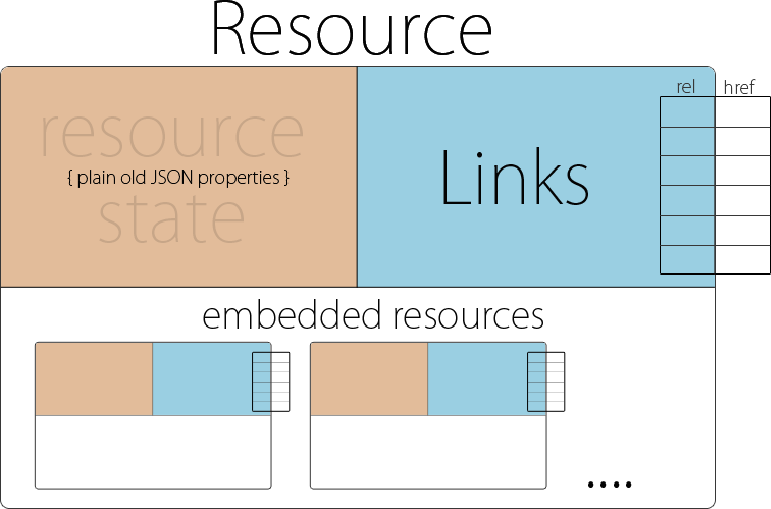
\includegraphics{images/hal}
\caption{Schéma zdroje ve formátu HAL \autocite{hal}\label{pic:hal}}
\end{figure}

\subsubsection*{JSON-LD}\label{json-ld}

JSON-LD je formát pro serializaci prolinkovaných dat \autocite{jsonld}. Používá se mj. pro sémantický web a RDF data \autocite{jsonldrdf}, ale lze jej použít i pro REST API. Příklad můžete vidět \protect\hyperlink{code:jsonld}{v~ukázce}.

\begin{listing}[htbp]
\caption{{\label{code:jsonld}Příklad formátu JSON-LD \autocite{jsonld}}}
\begin{minted}[bgcolor=codebg]{python}
{
  "@context": "http://json-ld.org/contexts/person.jsonld",
  "@id": "http://dbpedia.org/resource/John_Lennon",
  "name": "John Lennon",
  "born": "1940-10-09",
  "spouse": "http://dbpedia.org/resource/Cynthia_Lennon"
}
\end{minted}
\end{listing}

\subsubsection*{Hydra (rozšíření JSON-LD)}\label{hydra-rozux161uxedux159enuxed-json-ld}

Hydra je rozšíření pro JSON-LD, které využívá speciální slovník vhodný pro webová API \autocite{hydra}.

\subsubsection*{JSON API}\label{json-api}

JSON API je specifikace pro webová API využívající JSON \autocite{jsonapi}. Jedná se o~velmi komplexní formát, který u~každého zdroje rozlišuje data, metadata, odkazy, vztahy a další prvky.

\subsubsection*{Collection+JSON}\label{collectionjson}

Collection+JSON je komplexní serializační formát postavený na JSONu určený pro kolekce dat \autocite{collectionjson}. Příklad můžete vidět \protect\hyperlink{code:collectionjson}{v~ukázce}.

\begin{listing}[htbp]
\caption{{\label{code:collectionjson}Příklad formátu Collection+JSON \autocite{collectionjson}}}
\begin{minted}[bgcolor=codebg]{python}
{ "collection" :
  {
    "version" : "1.0",
    "href" : "http://example.org/friends/",
    
    "links" : [
      {"rel" : "feed", "href" : "http://example.org/friends/rss"}
    ],

    "items" : [
      {
        "href" : "http://example.org/friends/jdoe",
        "data" : [
          {"name" : "full-name", "value" : "J. Doe",
           "prompt" : "Full Name"},
          {"name" : "email", "value" : "jdoe@example.org",
           "prompt" : "Email"}
        ],
        "links" : [
          {"rel" : "blog", "href" : "http://examples.org/blogs/jdoe",
          "prompt" : "Blog"},
          {"rel" : "avatar",
           "href" : "http://examples.org/images/jdoe",
           "prompt" : "Avatar", "render" : "image"}
        ]
      }
    ],

    "queries" : [
      {"rel" : "search", "href" : "http://example.org/friends/search",
       "prompt" : "Search",
        "data" : [
          {"name" : "search", "value" : ""}
        ]
      }
    ],

    "template" : {
      "data" : [
        {"name" : "full-name", "value" : "", "prompt" : "Full Name"},
        {"name" : "email", "value" : "", "prompt" : "Email"},
        {"name" : "blog", "value" : "", "prompt" : "Blog"},
        {"name" : "avatar", "value" : "", "prompt" : "Avatar"}
      ]
    }
  }
}
\end{minted}
\end{listing}

\subsubsection*{Siren}\label{siren}

Siren je specifikace pro reprezentaci entit pomocí hypermédií \autocite{siren}. Příklad můžete vidět \protect\hyperlink{code:siren}{v~ukázce}.

\begin{listing}[htbp]
\caption{{\label{code:siren}Příklad formátu Siren \autocite{siren}}}
\begin{minted}[bgcolor=codebg]{python}
{
  "class": [ "order" ],
  "properties": {
      "orderNumber": 42,
      "itemCount": 3,
      "status": "pending"
  },
  "entities": [
    {
      "class": [ "items", "collection" ],
      "rel": [ "http://x.io/rels/order-items" ],
      "href": "http://api.x.io/orders/42/items"
    },
    {
      "class": [ "info", "customer" ],
      "rel": [ "http://x.io/rels/customer" ],
      "properties": {
        "customerId": "pj123",
        "name": "Peter Joseph"
      },
      "links": [
        { "rel": [ "self" ],
          "href": "http://api.x.io/customers/pj123" }
      ]
    }
  ],
  "actions": [
    {
      "name": "add-item",
      "title": "Add Item",
      "method": "POST",
      "href": "http://api.x.io/orders/42/items",
      "type": "application/x-www-form-urlencoded",
      "fields": [
        { "name": "orderNumber", "type": "hidden", "value": "42" },
        { "name": "productCode", "type": "text" },
        { "name": "quantity", "type": "number" }
      ]
    }
  ],
  "links": [
    { "rel": [ "self" ], "href": "http://api.x.io/orders/42" },
    { "rel": [ "previous" ], "href": "http://api.x.io/orders/41" },
    { "rel": [ "next" ], "href": "http://api.x.io/orders/43" }
  ]
}
\end{minted}
\end{listing}

Vzhledem ke komplexitě možných případů nestanovuji škálu pevně, ale na základě vlastního textového hodnocení ohodnotím každý framework nula až třemi body.

\subsection{Přístupová práva}\label{pux159uxedstupovuxe1-pruxe1va}

Některé frameworky přístupová práva vůbec neřeší, jiné podporují jen autentizaci, ale ne různá práva pro různé klienty a různé zdroje, další obsahují mechanismy a postupy, jak autentizaci a autorizaci řešit. Některé dokonce obsahují předpřipravená řešení pro nejčastější případy, jako je HTTP autentizace uživatelským jménem a heslem nebo OAuth.

Vzhledem ke komplexitě možných případů nestanovuji škálu pevně, ale na základě vlastního textového hodnocení ohodnotím každý framework nula až třemi body.

\subsection{Použitelnost}\label{pouux17eitelnost}

Jak je framework použitelný a přívětivý pro programátora se velice špatně stanovuje. Jedná se víceméně o~subjektivní dojem; to, co jeden programátor považuje za přívětivé, jiný může považovat za příliš složité.

Místo vynášení soudů o~použitelnosti, založených čistě na mém osobním názoru, nabídnu u~každého frameworku ukázku z~dokumentace, aby čtenář mohl použitelnost sám posoudit.

Jednotlivé ukázky se liší délkou i účelem. Ukázky z~vybraných frameworků sloužící ke stejnému účelu najdete v~kapitole \emph{\nameref{implementace}}.

\subsection{Stav projektu}\label{stav-projektu}

Pokud se rozhodujeme, jestli využít nějaký framework, mohly by nás zajímat i informace o~projektu, jako například:

\begin{itemize}
\tightlist
\item
  Kdo projekt tvoří; jsou to jednotlivci, firma?
\item
  Je projekt aktivně vyvíjen?
\item
  Vycházejí nové verze?
\item
  Reaguje někdo na hlášené chyby?
\item
  Jsou přijímány úpravy od lidí mimo projekt?
\item
  Jak dlouho již projekt existuje?
\item
  Jak často vycházejí nové verze?
\item
  Má projekt dokumentaci? Je aktuální?
\end{itemize}

Tyto informace se dají jen velice těžko srovnávat pomocí číselné škály, proto se pokusím na tyto otázky odpovědět alespoň textově.

\section{Cornice}\label{cornice}

Cornice je RESTový framework pro Pyramid \autocite{cornice}. Je vyvíjen lidmi z~Mozilla Services a vydán pod Mozilla Public License 2.0 \autocite{mpl2}, čímž se řadí do kategorie LGPL. Závisí na dvou dalších modulech (\verb!pyramid! a \verb!simplejson!), čímž nepřímo závisí na celkem devíti modulech a má s~nimi 124~625 řádek kódu. Podporuje obě verze Pythonu. Na GitHubu má 270 hvězd a za poslední měsíc byl stažen více než desettisíckrát.

Projekt vznikl v~roce 2011 a od té doby vyšla již více než dvacítka verzí. V~době zkoumání byla nejnovější verze pouze několik týdnů stará, proto vývoj hodnotím jako aktivní. Na vývoji se podílelo více než šest desítek vývojářů, většina z~nich formou drobné úpravy, která bývá rychle přijata i od lidí mimo projekt a mimo Mozilla Services.

\protect\hyperlink{code:cornice}{V~ukázce kódu} najdete příklad použití Cornice. V~ukázce je definována služba, která umožňuje použít GET a POST na nějakou hodnotu \verb!/values/{value}!, kde \verb!value! reprezentuje ASCII název té hodnoty.

\begin{listing}[htbp]
\caption{{\label{code:cornice}Příklad použití z~dokumentace Cornice \autocite{cornicedoc}}}
\begin{minted}[bgcolor=codebg]{python}
from cornice import Service

values = Service(name='foo', path='/values/{value}',
                 description="Cornice Demo")

_VALUES = {}


@values.get()
def get_value(request):
    """Returns the value.
    """
    key = request.matchdict['value']
    return _VALUES.get(key)


@values.post()
def set_value(request):
    """Set the value.

    Returns *True* or *False*.
    """
    key = request.matchdict['value']
    try:
        # json_body is JSON-decoded variant of the request body
        _VALUES[key] = request.json_body
    except ValueError:
        return False
    return True
\end{minted}
\end{listing}

\subsection{HATEOAS}\label{hateoas}

Cornice nenabízí předem připravené mechanismy k~prolinkování zdrojů. Pokud chcete použít JSON API, HAL či další obdobné standardy, budete je muset dodržet a naimplementovat sami. Cornice nezískává žádný bod.

\subsection{Přístupová práva}\label{pux159uxedstupovuxe1-pruxe1va}

Cornice nenabízí žádné zabudované možnosti, jak řešit přístupová práva. Ve výchozím stavu je celé API přístupné všem, můžete však napsat vlastní funkci v~Pythonu, která práva bude řešit. Toto na jednu stranu nabízí téměř neomezené možnosti, na stranu druhou to není příliš pohodlné. Cornice získává jeden bod.

Cornice působí jako solidní nízkoúrovňový REST framework: Pokud víte, co děláte, můžete pomocí něj naimplementovat REST službu, ale neudělá příliš věcí za vás. Speciální funkcí je pak podpora SPORE\footnote{Specification to a POrtable Rest Environment \autocite{spore}} \autocite{cornicespore}.
 \section{\texorpdfstring{Django REST framework \label{drf:fra}}{Django REST framework }}\label{django-rest-framework}

Django REST framework je nadstavbou k~webovému frameworku Django. Na svém webu \autocite{djangorest} uvádí tyto přednosti:

\begin{itemize}
\tightlist
\item
  webově procházetelné API (ukázku můžete vidět na \protect\hyperlink{pic:djangorestbrowsable}{na obrázku}),
\item
  autentizační pravidla včetně možnosti použití OAuth 1 či OAuth 2,
\item
  serializace pro ORM\footnote{Object-relational mapping neboli Objektově relační zobrazení \autocite{ormbook}} i jiná data,
\item
  upravitelné na míru,
\item
  rozsáhlá dokumentace a výborná komunitní podpora,
\item
  používají ho i velké společnostmi jako Mozilla a Eventbrite.
\end{itemize}

\begin{figure}
\centering

\includegraphics{images/django-rest-framework}
\caption{Logo Django REST frameworku \autocite{djangorest}\label{pic:djangorest}}
\end{figure}

\begin{figure}
\centering
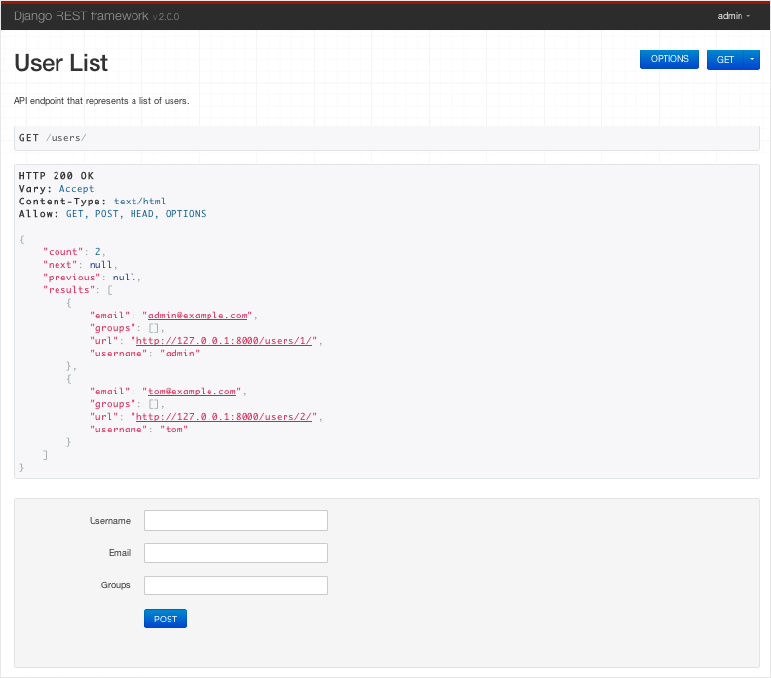
\includegraphics{images/django-rest-framework-browsable}
\caption{Django REST framework: Webově procházetelné API \autocite{djangorest}\label{pic:djangorestbrowsable}}
\end{figure}

Za vývojem Django REST frameworku nestojí žádná firma, ale jednotlivec, Tom Christie. Kromě něj ale do projektu přispělo více než pět set přispěvatelů \autocite{djangorestcontributors}. Projekt navíc absolvoval crowdfundingovou kampaň a podpořilo jej mnoho firem i jednotlivců \autocite{djangorestkickstarter}. Zveřejněn je podobně jako Django pod BSD licencí \autocite{BSD2}.

Příklad použití z~dokumentace, mírně upravený, aby se vešel na stránku, najdete \protect\hyperlink{code:djangorest}{v~ukázce}.

\begin{listing}[htbp]
\caption{{\label{code:djangorest}Příklad použití z~dokumentace Django REST frameworku \autocite{djangorestdoc}}}
\begin{minted}[bgcolor=codebg]{python}
# Serializers
from django.contrib.auth.models import User, Group
from rest_framework import serializers

class UserSerializer(serializers.HyperlinkedModelSerializer):
    class Meta:
        model = User
        fields = ('url', 'username', 'email', 'groups')

class GroupSerializer(serializers.HyperlinkedModelSerializer):
    class Meta:
        model = Group
        fields = ('url', 'name')

# Views
from django.contrib.auth.models import User, Group
from rest_framework import viewsets
from tutorial.quickstart.serializers import UserSerializer
from tutorial.quickstart.serializers import GroupSerializer

class UserViewSet(viewsets.ModelViewSet):
    """
    API endpoint that allows users to be viewed or edited.
    """
    queryset = User.objects.all().order_by('-date_joined')
    serializer_class = UserSerializer

class GroupViewSet(viewsets.ModelViewSet):
    """
    API endpoint that allows groups to be viewed or edited.
    """
    queryset = Group.objects.all()
    serializer_class = GroupSerializer

# URLs
from django.conf.urls import url, include
from rest_framework import routers
from tutorial.quickstart import views

router = routers.DefaultRouter()
router.register(r'users', views.UserViewSet)
router.register(r'groups', views.GroupViewSet)

# Wire up our API using automatic URL routing.
# Additionally, we include login URLs for the browsable API.
urlpatterns = [
    url(r'^', include(router.urls)),
    url(r'^api-auth/', include('rest_framework.urls',
                               namespace='rest_framework'))
]
\end{minted}
\end{listing}

První verze byla vydána již v~roce 2011 a od té doby jich vyšlo celkem osmdesát; poslední cca tři týdny před psaním tohoto textu. Vývoj je velmi aktivní a dokumentace obsáhlá. Instalace závisí pouze na Djangu, které nemá žádné další závislosti, a společně s~ním má 79~854 řádků kódu. Podporovány jsou obě verze Pythonu. Na GitHubu má více než pět a půl tisíce hvězd a za poslední měsíc byl více než třistatisíckrát stažen z~PyPI.

\subsection{HATEOAS}\label{hateoas}

Dokumentace obsahuje kapitolu o~HATEOAS \autocite{djangoresthateoas}, která uvádí:

\begin{quote}
Je zřejmé, že (Django) REST framework umožňuje vytvářet Hypermedia API. Procházetelné API, které nabízí, je postaveno na HTML -- jazyku hypermédií webu.

(Django) REST framework také obsahuje serializační, parsovací a renderovací komponenty usnadňující vytváření patřičných mediálních typů, hyperlinkovaných vazeb pro konstrukci vysoce propojených systémů, a dobrou podporu pro vyjednávání obsahu.

Co ale (Django) REST framework neumí, je vytváření strojově čitelných formátů hypermédií jako HAL, Collection+JSON, JSON API či HTML mikroformátů ve výchozí konfiguraci, či automagické generování plně HATEOAS API s~hypermediálním popisem formulářů a sémanticky označenými hyperlinky. To by vyžadovalo provedení takových rozhodnutí o~designu API, která by ve skutečnosti měla zůstat vně pole působnosti tohoto frameworku.
\end{quote}

Hodnotím kladně, že se o~principu HATEOAS v~dokumentaci hovoří. Prolinkování zdrojů ve stylu HATEOAS je v~Django REST frameworku jednoduché. Naplnění konkrétních implementací však zůstává v~režii architekta či programátora; Django REST framework k~tomu poskytuje dostatečné možnosti, uděluji mu tedy tři body.

\subsection{Přístupová práva}\label{pux159uxedstupovuxe1-pruxe1va}

Django REST framework umožňuje jak různé způsoby autentizace \autocite{djangorestauth}, tak i autorizace \autocite{djangorestperm}. V~základu poskytuje autentizaci:

\begin{itemize}
\tightlist
\item
  uživatelským jménem a heslem,
\item
  tokenem,
\item
  pomocí session.
\end{itemize}

Zároveň je možné implementovat vlastní způsoby. Existují další Python moduly, které tuto možnost využívají a přidávají tak do Django REST frameworku další možnosti autentizace, mezi ty nejdůležitější patří moduly pro OAuth~1 i OAuth~2. Například Django REST framework OAuth je modul, který byl dříve součástí Django REST frameworku, ale nyní je spravován samostatně.

Přístupová práva je možné řešit na úrovni objektů, modelů či konkrétních pohledů, tedy vlastně na základě URL. Pro první dvě kategorie se používají zabudované mechanismy přímo z~Djanga. Jsou rozlišena práva pro čtení a pro zápis. Stejně jako u~autentizace, i zde je možné si napsat vlastní způsob rozhodování přístupových práv a i zde vzniklo několik modulů třetích stran.

Možností poskytuje mnoho, Django REST framework tedy dostává i zde tři body.

Celkově Django REST framework působí jako obsáhlý nástroj poskytující mnoho možností a funkcí. Jeho jedinou zjevnou slabinou je těsná provázanost s~Djangem.
 \section{Eve}\label{eve}

\begin{figure}
\centering
\includegraphics{pdfs/eve}
\caption{Logo Eve \autocite{evepic}\label{pic:eve}}
\end{figure}

Eve je open-source REST API framework navržený „pro lidi“. Umožňuje snadno vytvořit a nasadit vysoce upravitelné, plně funkční RESTful webové služby. Eve stojí nad nástroji Flask, Redis, Cerberus, Events a podporuje MongoDB i SQL backendy. \autocite{eve}

Eve vychází z~následujícího principu: Máte nějaká data a chcete k~nim vytvořit REST API, pokud možno co nejvíce automaticky. Prakticky bez práce nabízí mj. tyto funkce a možnosti \autocite{eveslides}:

\begin{itemize}
\tightlist
\item
  filtrování,
\item
  řazení,
\item
  stránkování,
\item
  projekce,
\item
  vnořené zdroje,
\item
  JSON nebo XML serializaci,
\item
  HATEOAS,
\item
  ukládání souborů,
\item
  limitování přístupu,
\item
  cache,
\item
  hromadné vkládání,
\item
  kontrolu integrity (pomocí ETagu),
\item
  validaci dat,
\item
  GeoJSON,
\item
  autentizaci a autorizaci,
\item
  podporu obou verzí Pythonu i PyPy,
\item
  verzování API,
\item
  generovanou dokumentaci.
\end{itemize}

Jak vidno, možností poskytuje opravdu mnoho. Příklad použití si můžete prohlédnout \protect\hyperlink{code:eve}{v~ukázce kódu}.

\begin{listing}[htbp]
\caption{{\label{code:eve}Příklad použití z~dokumentace Eve \autocite{evedoc}}}
\begin{minted}[bgcolor=codebg]{python}
# run.py
from eve import Eve
app = Eve()

if __name__ == '__main__':
    app.run()


# settings.py
DOMAIN = {'people': {}}


# GET /
{
    "_info": {
        "server": "Eve",
        "version": "a.b.c",
        "api_version": "x.y.z"
    },
    "_links": {
        "child": [
            {
                "href": "people",
                "title": "people"
            }
        ]
    }
}


# GET /people
{
    "_items": [],
    "_links": {
        "self": {
            "href": "people",
            "title": "people"
        },
        "parent": {
            "href": "/",
            "title": "home"
        }
    }
}
\end{minted}
\end{listing}

Projekt vznikl v~roce 2012, od té doby vyšlo dvacet verzí, poslední cca tři týdny před psaním tohoto textu. Jedná se tedy o~aktivní projekt. Stojí za ním jednotlivec, Nicola Iarocci, a přispělo do něj více než sto dalších přispěvatelů \autocite{evecontributors}. Eve je vydáno pod BSD licencí \autocite{BSD3}.

Eve závisí celkem na deseti modulech (včetně Flasku a Werkzeugu) a tyto moduly již nemají žádné další závislosti. Celkem se závislostmi má 35~009 řádků kódu. Závislost na Python modulech pro MongoDB bohužel není volitelná.

\subsection{HATEOAS}\label{hateoas}

Eve automaticky prolinkovává jednotlivé zdroje a drží se konceptu HATEOAS \autocite{evehateoas}. Tuto funkci není potřeba speciálně nastavovat ani implementovat, je implicitně zapnutá. Každá odpověď na metodu GET obsahuje položku \verb!_links! s~odkazy na rodiče, subsekce, předchozí a další stránky apod. Příklad můžete vidět \protect\hyperlink{code:evehateoas}{v~ukázce}.

Autoři pracují na přímé podpoře pro JSON-LD, HAL i Siren \autocite{eveslides}.

V~této oblasti Eve hodnotím třemi body.

\begin{listing}[htbp]
\caption{{\label{code:evehateoas}Příklad HATEOAS principu z~Eve \autocite{evehateoas}}}
\begin{minted}[bgcolor=codebg]{python}
{
    "_links": {
        "self": {
            "href": "people",
            "title": "people"
        },
        "parent": {
            "href": "/",
            "title": "home"
        },
        "next": {
            "href": "people?page=2",
            "title": "next page"
        },
        "last": {
            "href": "people?page=10",
            "title": "last page"
        }
    }
}
\end{minted}
\end{listing}

\subsection{Přístupová práva}\label{pux159uxedstupovuxe1-pruxe1va}

Eve umožňuje několik způsobů autentizace, například pomocí tokenu nebo HMAC\footnote{Hash Message Authentication Code \autocite{hmac}} \autocite{eveauth}. Pomocí externích knihoven je snadné přidat i OAuth 2 \autocite{eveoauth}.

Eve umožňuje nastavovat přístupová práva podle rolí pro celé API, nebo jen pro některé zdroje, stejně tak pro konkrétní HTTP metody \autocite{eveauth}.

Dávám tedy i zde Eve tři body.

Celkově se Eve jeví jako framework s~mnoha funkcemi, který dokáže ušetřit velké množství práce. Vytknul bych snad jen přílišnou vázanost na MongoDB, která je často patrná především z~dokumentace.
 \section{Falcon}\label{falcon}

Falcon je neuvěřitelně rychlý, minimalistický Python webový framework pro tvorbu „cloudových API“ a aplikačních backendů \autocite{falcon}. Mezi hlavní přednosti podle webové stránky \autocite{falcon} patří:

\begin{itemize}
\tightlist
\item
  závislost pouze na modulech \verb!six! a \verb!mimeparse!,
\item
  rychlejší zpracování požadavků než u~jiných populárních frameworků,
\item
  podpora WSGI, CPythonu 2.6, 2.7, 3.3 a 3.4 i PyPy,
\item
  svoboda volby detailů,
\item
  spolehlivost.
\end{itemize}

\begin{figure}
\centering

\includegraphics{images/falcon}
\caption{Logo Falconu \autocite{falconpic}\label{pic:falcon}}
\end{figure}

Falcon je bezesporu minimalistický -- společně se závislostmi má pouze 3~034 řádků kódu. Je šířen pod permisivní Apache licencí \autocite{apache} a nevyžaduje žádný webový framework.

Příklad použití můžete najít \protect\hyperlink{code:falcon}{v~ukázce}. Jak je vidět, pomocí Falconu jdou vytvářet REST API, ale jedná se o~velmi nízkoúrovňový framework, který spíše zastává vrstvu mezi HTTP a aplikací než velkého pomocníka při tvorbě API.

\begin{listing}[htbp]
\caption{{\label{code:falcon}Příklad použití z~webu Falconu \autocite{falcon}}}
\begin{minted}[bgcolor=codebg]{python}
# sample.py
import falcon
import json

class QuoteResource:
    def on_get(self, req, resp):
        """Handles GET requests"""
        quote = {
            'quote': 'I\'ve always been more interested '
                     'in the future than in the past.',
            'author': 'Grace Hopper'
        }

        resp.body = json.dumps(quote)

api = falcon.API()
api.add_route('/quote', QuoteResource())
\end{minted}
\end{listing}

Projekt vytváří firma Rackspace pod vedením Kurta Griffithse. Do projektu přispívají i jednotlivci mimo Rackspace. Vznikl v~roce 2012 a od té doby vyšlo celkem 27 verzí. Dva týdny před psaním tohoto textu vyšla verze 1.0.0rc1, brzy se tedy můžeme těšit na verzi 1.0.0. Jedná se o~aktivní projekt, který se může chlubit stoprocentním pokrytím testy \autocite{falconcoverage}.

Vzhledem k~nízkoúrovnosti frameworku neexistují žádné automatické mechanismy pro správu přístupových práv či HATEOAS. Falcon tedy za oba aspekty získává nula bodů.
 \section{\texorpdfstring{hug (rozšíření pro Falcon) \label{hug}}{hug (rozšíření pro Falcon) }}\label{hug-rozux161uxedux159enuxed-pro-falcon}

Cílem hugu je, aby vytváření API v~Pythonu bylo co nejjednodušší. Pomocí hugu lze vytvářet API nejen pro HTTP, ale i pro další média, například CLI aplikace. \autocite{hugweb}

\begin{figure}
\centering

\includegraphics{images/hug}
\caption{Logo hugu \autocite{hugpic}\label{pic:hug}}
\end{figure}

Mezi hlavní cíle hugu patří \autocite{huggithub}:

\begin{itemize}
\tightlist
\item
  umožnit psaní tak stručného kódu Python API, jako by šlo o~psanou definici,
\item
  framework by měl podporovat psaní srozumitelného kódu,
\item
  měl by být dostatečně rychlý; vývojář by neměl mít potřebu se kvůli výkonu poohlížet jinam,
\item
  psaní testů pro API napsaná v~hugu by mělo být jednoduché a intuitivní,
\item
  magie by se měla odehrávat jen na jednom místě, ve frameworku, což je lepší než delegovat tento problém na uživatele,
\item
  být základním kamenem API nové generace, díky nejnovějším technologiím.
\end{itemize}

Kvůli poslednímu bodu je hug kompatibilní pouze s~Pythonem 3 a pro webová API staví na frameworku Falcon, o~kterém jsem psal \protect\hyperlink{falcon}{v~části} \autocite{huggithub}.

Příklad použití s~využitím typové anotace dostupné od Pythonu 3.5 můžete vidět \protect\hyperlink{code:hug}{v~ukázce}.

\begin{listing}[htbp]
\caption{{\label{code:hug}Příklad použití z~dokumentace hugu \autocite{hugdoc}}}
\begin{minted}[bgcolor=codebg]{python}
"""First hug API (local and HTTP access)"""
import hug


@hug.get(examples='name=Timothy&age=26')
@hug.local()
def happy_birthday(name: hug.types.text, age: hug.types.number,
                   hug_timer=3):
    """Says happy birthday to a user"""
    return {'message': 'Happy {0} Birthday {1}!'.format(age, name),
            'took': float(hug_timer)}


# GET /happy_birthday?name=Timothy&age=26
{
    "took": 0,
    "message": "Happy 26 Birthday Timothy"
}

# GET /happy_birthday?name=Timothy
{
    "errors": {
        "age": "Required parameter not supplied"
    }
}

# GET /happy_birthday?name=Timothy&age=twentysix
{
    "errors": {
        "age": "Invalid whole number provided"
    }
}
\end{minted}
\end{listing}

Hug je mladý projekt, vznikl teprve v~červenci roku 2015. Více než tři tisíce hvězd na GitHubu za tak krátkou dobu ale napovídá, že půjde o~projekt oblíbený; z~PyPI byl stažen za poslední měsíc více než sedmtisíckrát. Vývoj probíhá docela rapidně, již vyšlo více než čtyřicet verzí, průměrně tedy vychází rychleji než jednou týdně. Na to doplácí především dokumentace, která zdaleka neobsahuje všechny možnosti hugu; postrádá například kapitolu o~autentizaci, přestože v~kódu je tato funkcionalita obsažena. Za projektem stojí jednotlivec Timothy Edmund Crosley, ale přispěla již třicítka vývojářů.

Hug je zveřejněn pod MIT licencí \autocite{MIT}. Přímo závisí na Falconu a knihovně Requests, nepřímo tak má 4 závislosti a společně s~nimi 16~545 řádků kódu.

\subsection{HATEOAS}\label{hateoas}

Hug bohužel zatím nepodporuje žádné automatické způsoby pro prolinkování jednotlivých zdrojů, nedostává tedy žádný bod.

\subsection{Přístupová práva}\label{pux159uxedstupovuxe1-pruxe1va}

Jak již bylo zmíněno výše, o~přístupových právech dokumentace mlčí. Z~pohledu do kódu \autocite{hugauth} je však patrné, že podporuje autentizaci pomocí:

\begin{itemize}
\tightlist
\item
  HTTP Basic (jménem a heslem),
\item
  API klíče v~HTTP hlavičce,
\item
  tokenu v~HTTP hlavičce.
\end{itemize}

O~autorizaci jsem však v~kódu nic nenašel, proto dávám hugu pouze dva body.

Hug je moderní framework pro vytváření různých API v~Pythonu. Jeho filozofie je rozhodně zajímavá, ale v~současnosti jej hodnotím jako příliš mladý a zatím stále se rozvíjející projekt.
 \section{Flask API}\label{flask-api}

Flask API je implementace stejných webově procházetelných API, které poskytuje Django REST framework \autocite{flaskapi} (o~něm jsem psal \protect\hyperlink{drf:fra}{v~části}), ale bez závislosti na Djangu.

Za projektem stojí autor Django REST frameworku, Tom Christie. Zatím se ale naneštěstí jedná o~rozdělanou práci \autocite{flaskapi} a zdaleka nejde o~hotový projekt. Práce na Flask API je zároveň pozastavená, kvůli závazkům z~crowdfundingové kapaně k~Django REST frameworku \autocite{flaskapigh}. Tom Christie se od roku 2014 (kdy projekt i vznikl) na projektu aktivně nepodílí, existují však další jednotlivci, kteří projekt udržují a rozvíjí.

Pomocí Flask API je nyní možné webově procházet API, jak můžete vidět \protect\hyperlink{pic:flaskapibrowsable}{na obrázku}, ale tvorba API zatím není příliš automatizovaná, \protect\hyperlink{code:flaskapi}{viz příklad}\footnote{Příklad byl mírně zhuštěn za účelem lepší prezentace na straně formátu A4.}.

\begin{figure}
\centering
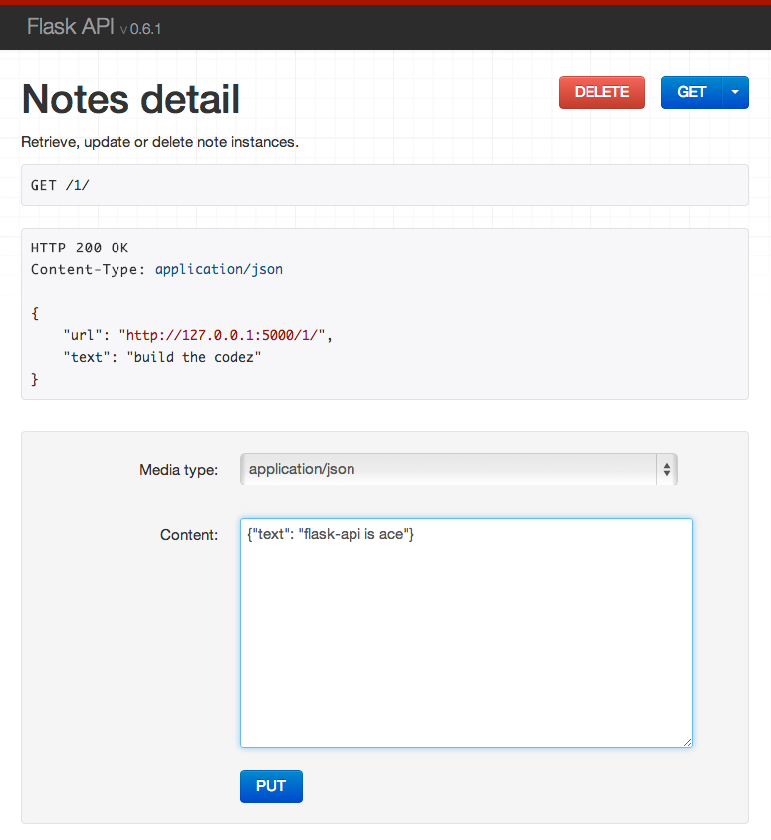
\includegraphics{images/flask-api-browsable}
\caption{Flask API: Webově procházetelné API \autocite{flaskapi}\label{pic:flaskapibrowsable}}
\end{figure}

\begin{listing}[htbp]
\caption{{\label{code:flaskapi}Příklad použití z~dokumentace Flask API \autocite{flaskapigh}}}
\begin{minted}[bgcolor=codebg]{python}
from flask import request, url_for
from flask_api import FlaskAPI, status, exceptions

app = FlaskAPI(__name__)

notes = {
    0: 'do the shopping',
    1: 'build the codez',
    2: 'paint the door',
}

def note_repr(key):
    return {
        'url': request.host_url.rstrip('/') + \
               url_for('notes_detail', key=key),
        'text': notes[key]
    }

@app.route("/", methods=['GET', 'POST'])
def notes_list():
    """List or create notes."""
    if request.method == 'POST':
        note = str(request.data.get('text', ''))
        idx = max(notes.keys()) + 1
        notes[idx] = note
        return note_repr(idx), status.HTTP_201_CREATED

    # request.method == 'GET'
    return [note_repr(idx) for idx in sorted(notes.keys())]

@app.route("/<int:key>/", methods=['GET', 'PUT', 'DELETE'])
def notes_detail(key):
    """Retrieve, update or delete note instances."""
    if request.method == 'PUT':
        note = str(request.data.get('text', ''))
        notes[key] = note
        return note_repr(key)

    elif request.method == 'DELETE':
        notes.pop(key, None)
        return '', status.HTTP_204_NO_CONTENT

    # request.method == 'GET'
    if key not in notes:
        raise exceptions.NotFound()
    return note_repr(key)

if __name__ == "__main__":
    app.run(debug=True)
\end{minted}
\end{listing}

Projekt v~současnosti přímo závisí jen na frameworku Flask, tím má nepřímo pět závislostí a s~nimi 20~938 řádků kódu. Je distribuován pod BSD licencí \autocite{BSD2} a podporuje obě verze Pythonu.

Do budoucna je plánováno \autocite{flaskapi}\autocite{flaskapigh}:

\begin{itemize}
\tightlist
\item
  autentizace, mj. pomocí session, tokenu i jménem a heslem,
\item
  přístupová práva,
\item
  limitování počtu požadavků v~čase,
\item
  API zdroje pomocí tříd,
\item
  vylepšení procházetelných API, například přidání drobečkové navigace,
\item
  možnost vlastního zpracování výjimek,
\item
  ochrana proti CSRF,
\item
  přihlašování a odhlašování přes prohlížeč v~případě procházetelných API,
\item
  zdokumentování validace požadavků a prolinkování.
\end{itemize}

Je však otázka, kdy a jestli se toho dočkáme.

Zatím neexistují žádné automatické mechanismy pro správu přístupových práv či HATEOAS. Flask API tedy za oba aspekty získává nula bodů.
 \section{Flask-RESTful}\label{flask-restful}

\begin{figure}
\centering

\includegraphics{images/flask-restful}
\caption{Logo Flask-RESTful \autocite{flaskresfulpic}\label{pic:flaskresful}}
\end{figure}

Flask-RESTful je rozšíření Flasku, které přidává podporu pro rychlé vytváření RESTových API. Jedná se o~tenkou vrstvu abstrakce, která by měla fungovat s~existujícím ORM a dalšími knihovnami. Flask-RESTful je navržen tak, aby ho uživatelé obeznámení s~Flaskem co nejrychleji pochopili. \autocite{flaskresful}

Za vývojem Flask-RESTful stojí firma Twilio, ale přispělo do něj více než sto jednotlivců. Je zveřejněn pod BSD licencí \autocite{BSD3}. Závisí na Flasku a dalších třech modulech. Celkově tak nepřímo závisí na modulech devíti a společně s~nimi má 27~718 řádků kódu. Na GitHubu má necelé dva tisíce hvězd a na PyPI má za poslední měsíc více než 170 tisíc stažení. Podporuje obě verze Pythonu. Projekt vznikl v~roce 2012, od té doby vyšlo 27 verzí, poslední v~prosinci roku 2015.

Příklad použití můžete vidět \protect\hyperlink{code:flaskresful}{v~ukázce}\footnote{Příklad byl mírně zhuštěn za účelem lepší prezentace na straně formátu A4.}.

\begin{listing}[htbp]
\caption{{\label{code:flaskresful}Příklad použití z~dokumentace Flask-RESTful \autocite{flaskrestfuldoc}}}
\begin{minted}[bgcolor=codebg]{python}
from flask import Flask
from flask_restful import reqparse, abort, Api, Resource

app = Flask(__name__)
api = Api(app)

TODOS = {'todo1': {'task': 'build an API'}, ...}

def abort_if_todo_doesnt_exist(todo_id):
    if todo_id not in TODOS:
        abort(404, message="Todo {} doesn't exist".format(todo_id))

parser = reqparse.RequestParser()
parser.add_argument('task')

# shows a single todo item and lets you delete a todo item
class Todo(Resource):
    def get(self, todo_id):
        abort_if_todo_doesnt_exist(todo_id)
        return TODOS[todo_id]

    def delete(self, todo_id):
        abort_if_todo_doesnt_exist(todo_id)
        del TODOS[todo_id]
        return '', 204

    def put(self, todo_id):
        args = parser.parse_args()
        task = {'task': args['task']}
        TODOS[todo_id] = task
        return task, 201

# shows a list of all todos, and lets you POST to add new tasks
class TodoList(Resource):
    def get(self):
        return TODOS

    def post(self):
        args = parser.parse_args()
        todo_id = int(max(TODOS.keys()).lstrip('todo')) + 1
        todo_id = 'todo%i' % todo_id
        TODOS[todo_id] = {'task': args['task']}
        return TODOS[todo_id], 201

# Actually setup the Api resource routing here
api.add_resource(TodoList, '/todos')
api.add_resource(Todo, '/todos/<todo_id>')

if __name__ == '__main__':
    app.run(debug=True)
\end{minted}
\end{listing}

Flask-RESTful je nízkoúrovňový framework, který zjednodušuje tvorbu REST API oproti použití čistého Flasku, ale nepřináší žádné pokročilé funkce jako podporu autentizace a autorizace, či prolinkování a HATEOAS. Nedostává tedy žádné body. Ze zajímavých funkcí Flask-RESTful mohu jmenovat vyjednávání o~obsahu či podporu \emph{blueprintů} (koncept z~Flasku \autocite{blueprint}).
 \section{Morepath}\label{morepath}

\begin{figure}
\centering

\includegraphics{images/morepath}
\caption{Koncept loga Morepathu \autocite{morepathpic}\label{pic:morepath}}
\end{figure}

Morepath je webový mikroframework podobně jako Flask nebo Bottle \autocite{morepath}. Nepatří tak úplně mezi frameworky na vytváření RESTových API, zařadil jsem jej proto, že přímo v~sobě obsahuje součásti pro jejich tvorbu \autocite{morepathrest}. Na rozdíl od jiných mikroframeworků je modelově orientovaný \autocite{morepath}.

Projekt vznikl v~roce 2013, ale jeho historie sahá dále do minulosti \autocite{morepathhistory}. Od roku 2013 vyšlo téměř dvacet verzí, poslední tři dny před psaním tohoto textu. Morepath přímo závisí na čtyřech a nepřímo na pěti modulech, společně s~nimi má 9~156 řádků kódu. Je distribuován pod BSD licencí \autocite{BSD3}. Autorem projektu je Martijn Faassen z~firmy CONTACT Software a přispělo do něj celkem 14 vývojářů. 226 hvězd na GitHubu a malý počet přispěvatelů dává tušit, že se nejedná o~příliš slavný projekt, obsahuje však mnoho zajímavých funkcí \autocite{morepathsp}.

V~případě RESTu jde hlavně o~jednoduché prolinkování v~duchu HATEOAS, které můžete vidět \protect\hyperlink{code:morepath}{v~ukázce}. Komplexnější příklad dokumentace neobsahuje. Morepath dostává za HATEOAS dva body.

Za účelem vytvoření webové služby je potřeba použít modely; to mohou být v~Morepathu objekty v~paměti, abstrakce databázových tabulek pomocí ORM, či data uložená v~NoSQL databázi.

\begin{listing}[htbp]
\caption{{\label{code:morepath}Příklad použití z~dokumentace Morepathu \autocite{morepathrest}}}
\begin{minted}[bgcolor=codebg]{python}
@App.json(model=DocumentCollection)
def collection_default(self, request):
    return {
       'type': 'document_collection',
       'documents': [dict(id=doc.id, link=request.link(doc))
                     for doc in self.documents],
       'add': request.link(documents, 'add')
    }
\end{minted}
\end{listing}

Přístupová práva umí Morepath nastavovat na úrovni modelů či pohledů a autentizace uživatele může proběhnout na základě session \autocite{morepathauth}. O~žádných speciálních metodách autentizace v~případě API se dokumentace nezmiňuje, dostává tedy jeden bod.

Hodnotím Morepath jako zajímavý webový mikroframewrok, pokud uživatel touží po modelech, ale nechce použít „velký“ MVC framework jako Django. Poskytnutím mechanismů pro tvorbu RESTful API přímo v~základu frameworku se řadí mezi ojedinělé Python webové frameworky.
 \section{Nefertari}\label{nefertari}

Nefertari je REST API framework pro Pyramid, který používá Elasticsearch pro čtení a MongoDB nebo PostgreSQL pro zápis \autocite{nefertari}.

V~Nefertari je nejprve potřeba připravit model, což je entita mapovaná na databázi, a k~danému modelu vytvořit pohled, což je mapování dané entity na HTTP metody. Ukázkový model a pohled můžete vidět \protect\hyperlink{code:nefertarimodel}{v~ukázkách} \protect\hyperlink{code:nefertariview}{a}. Serializaci do JSONu a mapování na URL za vás obstará framework.

\begin{listing}[htbp]
\caption{{\label{code:nefertarimodel}Příklad použití z~dokumentace Nefertari (model) \autocite{nefertarimodel}}}
\begin{minted}[bgcolor=codebg]{python}
from datetime import datetime
from nefertari import engine as eng
from nefertari.engine import BaseDocument


class Story(BaseDocument):
    __tablename__ = 'stories'

    _auth_fields = [
        'id', 'updated_at', 'created_at', 'start_date',
        'due_date', 'name', 'description']
    _public_fields = ['id', 'start_date', 'due_date', 'name']

    id = eng.IdField(primary_key=True)
    updated_at = eng.DateTimeField(onupdate=datetime.utcnow)
    created_at = eng.DateTimeField(default=datetime.utcnow)

    start_date = eng.DateTimeField(default=datetime.utcnow)
    due_date = eng.DateTimeField()

    name = eng.StringField(required=True)
    description = eng.TextField()
\end{minted}
\end{listing}

\begin{listing}[htbp]
\caption{{\label{code:nefertariview}Příklad použití z~dokumentace Nefertari (pohled) \autocite{nefertariview}}}
\begin{minted}[bgcolor=codebg]{python}
from nefertari.view import BaseView
from example_api.models import Story


class StoriesView(BaseView):
    Model = Story

    def index(self):
        return self.get_collection_es()

    def show(self, **kwargs):
        return self.context

    def create(self):
        story = self.Model(**self._json_params)
        return story.save(self.request)

    def update(self, **kwargs):
        story = self.Model.get_item(
            id=kwargs.pop('story_id'), **kwargs)
        return story.update(self._json_params, self.request)

    def replace(self, **kwargs):
        return self.update(**kwargs)

    def delete(self, **kwargs):
        story = self.Model.get_item(
            id=kwargs.pop('story_id'), **kwargs)
        story.delete(self.request)

    def delete_many(self):
        es_stories = self.get_collection_es()
        stories = self.Model.filter_objects(es_stories)

        return self.Model._delete_many(stories, self.request)

    def update_many(self):
        es_stories = self.get_collection_es()
        stories = self.Model.filter_objects(es_stories)

        return self.Model._update_many(
            stories, self._json_params, self.request)
\end{minted}
\end{listing}

Nefertari závisí na devíti, nepřímo na osmnácti modulech, což je oproti jiným zkoumaným frameworkům opravdu hodně. Instalace obsahuje celkem 54~339 řádků kódu. Podporován je Python 2 i 3. Projekt je distribuován pod permisivní Apache licencí \autocite{apache}.

První commit v~projektu se datuje na březen 2015, jedná se tedy, v~době psaní tohoto textu, zhruba o~jeden rok starý projekt. Od té doby vyšlo téměř patnáct verzí, poslední v~listopadu 2015. Za projektem stojí startup Brandicted\footnote{Hlavní služba startupu Brandicted.com je v~době psaní tohoto textu nedostupná. Je otázkou, zdali jde o~náhodu, nebo má Nefertari nejistou budoucnost. Repozitář na GitHubu (který má 37 hvězd) se přesunul do organizace \emph{ramses-tech}, která ale obsahuje stejné vývojáře jako původní organizace \emph{brandicted}.}, kromě nich do projektu příliš mnoho lidí nepřispívá.

\subsection{HATEOAS}\label{hateoas}

Dokumentace Nefertari se nezmiňuje o~způsobu, jak jednotlivé zdroje prolinkovat. V~části \emph{Vize} \autocite{nefertarivision} dokonce přímo říká:

\begin{quote}
Pro nás znamená „REST API“ něco jako „HTTP metody namapované na CRUD\footnote{\emph{Create}, \emph{Retrieve}, \emph{Update}, \emph{Delete}} operace nad zdroji popsanými v~JSONu“. Nesnažíme se o~úplný HATEOAS, ani o~naplnění akademického ideálu o~RESTu.
\end{quote}

Nedostává tedy žádné body.

\subsection{Přístupová práva}\label{pux159uxedstupovuxe1-pruxe1va}

Nefertari používá model autentizace z~frameworku Pyramid, pomocí cookies \autocite{nefertariauth}, což je pro REST API nevyhovující. Přístupová práva oproti tomu umožňuje nastavit velice variabilně na úrovni jednotlivých operací a zdrojů \autocite{nefertariauth}. Dostává tedy jeden bod.

Nefertari vede k~tomu, že se vývojář o~některé věci vůbec nemusí starat: jak přesně jsou data uložena v~databázi nebo jak se mapují zdroje na URL. To může být velkou výhodou, ale i nevýhodou. Podle dokumentace se zdá, že jednotlivá výchozí chování nelze příliš ovlivnit. Nefertari jistě ušetří mnoho práce za cenu svobody volby. Absence HATEOAS a autentizace pomocí cookies můj pohled na Nefertari příliš nezlepší. Existují jistě situace, kde bude Nefertari velmi vhodná, ale není dostatečně flexibilní pro širokou škálu případů.
 \section{Ramses (rozšíření pro Nefertari)}\label{ramses-rozux161uxedux159enuxed-pro-nefertari}

\begin{figure}
\centering
\includegraphics{pdfs/ramses}
\caption{Logo Ramsesu \autocite{ramses}\label{pic:ramses}}
\end{figure}

Ramses je framework, který generuje RESTful API pomocí RAMLu \footnote{\emph{RESTful API Modeling Language}, postavený na YAMLu \autocite{raml}}. Používá Pyramid a Nefertari \autocite{ramsesdoc}.

Ramses přináší stejné funkce jako Nefertari, o~které jsem psal \protect\hyperlink{nefertari}{v~části}. Místo kódu v~Pythonu se však používá deskriptivní jazyk RAML.

Ramses přímo závisí na sedmi modulech, nepřímo pak na téměř třiceti, instalace má celkem 68~594 řádků kódu. V~počtu závislostí je tak v~negativním slova smyslu vítězem.

Projekt vytváří stejní autoři jako Nefertari a všechny informace o~aktivitě jsou prakticky stejné. Projekt vznikl na přelomu února a března 2015, poslední z~dvanácti verzí vyšla v~listopadu téhož roku. Kód je distribuován pod permisivní Apache licencí \autocite{apache}, stejně jako Nefertari. Na rozdíl od Nefertari má na GitHubu více než dvě stovky hvězd.

Zkrácený příklad RAML souboru pro vytvoření API můžete vidět \protect\hyperlink{code:ramses}{v~ukázce}. V~odpovědi \protect\hyperlink{code:ramsesreply}{v~ukázce} pak můžete vidět absenci prolinkování.

\begin{listing}[htbp]
\caption{{\label{code:ramses}Příklad použití Ramsesu \autocite{ramsespizza}}}
\begin{minted}[bgcolor=codebg]{yaml}
#%RAML 0.8
---
title: pizza_factory API
documentation:
    - title: pizza_factory REST API
      content: |
        Welcome to the pizza_factory API.
baseUri: http://{host}:{port}/{version}
version: v1
mediaType: application/json
protocols: [HTTP]

/cheeses:
    displayName: Collection of different cheeses
    get:
        description: Get all cheeses
    post:
        description: Create a new cheese
        body:
            application/json:
                schema: !include schemas/cheeses.json

    /{id}:
        displayName: A~particular cheese ingredient
        get:
            description: Get a particular cheese
        delete:
            description: Delete a particular cheese
        patch:
            description: Update a particular cheese

/pizzas:
    displayName: Collection of pizza styles
    get:
        description: Get all pizza styles
    post:
        description: Create a new pizza style
        body:
            application/json:
                schema: !include schemas/pizzas.json

    /{id}:
        displayName: A~particular pizza style
        get:
            description: Get a particular pizza style
        delete:
            description: Delete a particular pizza style
        patch:
            description: Update a particular pizza style

# ...
\end{minted}
\end{listing}

\begin{listing}[htbp]
\caption{{\label{code:ramsesreply}Odpověď Ramsesu \autocite{ramsespizza}}}
\begin{minted}[bgcolor=codebg]{python}
# POST /api/pizzas name=hawaiian toppings:=[1,2] ...
{
    "data": {
        "_type": "Pizza",
        "_version": 0,
        "cheeses": [
            1
        ],
        "crust": 1,
        "crust_id": 1,
        "description": null,
        "id": 1,
        "name": "hawaiian",
        "sauce": 1,
        "sauce_id": 1,
        "self": "http://localhost:6543/api/pizzas/1",
        "toppings": [
            1,
            2
        ],
        "updated_at": null
    },
    "explanation": "",
    "id": "1",
    "message": null,
    "status_code": 201,
    "timestamp": "2015-06-05T18:47:53Z",
    "title": "Created"
}
\end{minted}
\end{listing}

Vzhledem k~tomu, že Ramses je vrstva abstrakce nad Nefertari, nebudu zde opakovat sekce o~HATEOAS a přístupových právech, jelikož by byly prakticky stejné. Vytváření REST API pomocí RAML souborů je možná směr, kterým se v~budoucnu lidstvo vydá, ale bojím se, že na Ramsesu je třeba ještě zapracovat. Otázkou je, jestli bude dále vyvíjen.
 \section{Piston}\label{piston}

\begin{figure}
\centering

\includegraphics{images/piston}
\caption{Logo Pistonu \autocite{pistonpic}\label{pic:piston}}
\end{figure}

Piston je, respektive spíše byl, mini-framework pro Django určený pro vytváření RESTful API \autocite{piston}.

Piston je interně svázán s~Djangem a podle své dokumentace nabízí následující funkce \autocite{piston}:

\begin{itemize}
\tightlist
\item
  podporuje OAuth bez nutnosti použití další knihovny,
\item
  nevyžaduje vazbu na modely, umožňuje vytvářet nezávislé zdroje,
\item
  komunikuje pomocí JSONu, YAMLu, Python picklu a XML (a také pomocí HATEOAS),
\item
  jde o~Python knihovnu, kterou lze snadno použít,
\item
  respektuje a nabádá ke správnému využití HTTP protokolu (návratové kódy apod.),
\item
  má zabudovanou (volitelnou) validaci vstupů (pomocí Djanga), omezování počtu požadavků v~čase apod.,
\item
  podporuje streamování s~malým využitím paměti,
\item
  „neplete se do cesty“.
\end{itemize}

Projekt vnikl již v~roce 2008, tedy tři roky po zveřejnění Djanga samotného, pod záštitou Bitbucketu. V~roce 2010 jej však původní autor, Jesper Nøhr, přestal vyvíjet. Vývoje se následující rok ujal Joshua Ginsberg, který ale vydal jen dvě nové verze a vývoj na začátku roku 2012 taktéž opustil. Poslední vydaná verze 0.2.3 přidává podporu pro Django 1.4, nejvyšší podporovaná verze je tedy snad 1.5\footnote{Django vždy nejprve označí funkcionalitu k~odebrání, v~následující verzi ji označí jako zastaralou (\emph{deprecated}) a v~další verzi ji odstraní \autocite{djangorelease}. Současné podporované verze jsou 1.8 a 1.9.}. S~Djangem 1.6 nebo vyšším Piston nefunguje \autocite{piston16}. Kód rovněž obsahuje syntaxi nekompatibilní s~Pythonem 3. Piston je tedy jednoznačně mrtvý projekt.

Piston byl distribuován pod BSD licencí (není však jasné, jestli jde o~třípoložkovou \autocite{BSD3} nebo dvoupoložkovou \autocite{BSD2} variantu, projekt neuvádí celý text licence). Závisí pouze na Djangu a společně s~Djangem 1.5 má 75~311 řádků kódu.

Příklad použití z~dokumentace můžete vidět \protect\hyperlink{code:piston1}{v~ukázkách} \protect\hyperlink{code:piston2}{a}.

\begin{listing}[htbp]
\caption{{\label{code:piston1}Příklad použití z~dokumentace Pistonu (urls.py) \autocite{piston}}}
\begin{minted}[bgcolor=codebg]{python}
from django.conf.urls.defaults import *
from piston.resource import Resource
from piston.authentication import HttpBasicAuthentication

from myapp.handlers import BlogPostHandler, ArbitraryDataHandler

auth = HttpBasicAuthentication(realm="My Realm")
ad = { 'authentication': auth }

blogpost_resource = Resource(handler=BlogPostHandler, **ad)
arbitrary_resource = Resource(handler=ArbitraryDataHandler, **ad)

urlpatterns += patterns('',
    url(r'^posts/(?P<post_slug>[^/]+)/$', blogpost_resource), 
    url(r'^other/(?P<username>[^/]+)/(?P<data>.+)/$',
        arbitrary_resource), 
)
\end{minted}
\end{listing}

\begin{listing}[htbp]
\caption{{\label{code:piston2}Příklad použití z~dokumentace Pistonu (handlers.py) \autocite{piston}}}
\begin{minted}[bgcolor=codebg]{python}
import re

from piston.handler import BaseHandler
from piston.utils import rc, throttle

from myapp.models import Blogpost

class BlogPostHandler(BaseHandler):
    allowed_methods = ('GET', 'PUT', 'DELETE')
    fields = ('title', 'content',
              ('author', ('username', 'first_name')), 'content_size')
    exclude = ('id', re.compile(r'^private_'))
    model = Blogpost

    @classmethod
    def content_size(self, blogpost):
        return len(blogpost.content)

    def read(self, request, post_slug):
        post = Blogpost.objects.get(slug=post_slug)
        return post

    @throttle(5, 10*60) # allow 5 times in 10 minutes
    def update(self, request, post_slug):
        post = Blogpost.objects.get(slug=post_slug)

        post.title = request.PUT.get('title')
        post.save()

        return post

    def delete(self, request, post_slug):
        post = Blogpost.objects.get(slug=post_slug)

        if not request.user == post.author:
            return rc.FORBIDDEN # returns HTTP 401

        post.delete()

        return rc.DELETED # returns HTTP 204

class ArbitraryDataHandler(BaseHandler):
    methods_allowed = ('GET',)

    def read(self, request, username, data):
        user = User.objects.get(username=username)

        return { 'user': user, 'data_length': len(data) }
\end{minted}
\end{listing}

\subsection{HATEOAS}\label{hateoas}

Přestože o~sobě Piston říká, že komunikuje pomocí HATEOAS principu \autocite{piston}, v~celé dokumentaci není nikde zmínka o~tom, jak z~jednoho zdroje linkovat zdroj jiný. Veškeré příklady místo linkování zobrazují další zdroj vnořeně, poměrně komplikovaným způsobem lze uvést alespoň ID \autocite{pistonid}. I~když by bylo možné si pro každý druh odkazu nadefinovat vlastní metodu, považuji to za zbytečně komplikované. Myslím, že použití zkraty HATEOAS je tedy v~popisu tohoto frameworku poměrně neoprávněné, a dávám nula bodů.

\subsection{Přístupová práva}\label{pux159uxedstupovuxe1-pruxe1va}

Piston nabízí dva druhy autentizace: základní HTTP autentizaci jménem a heslem a OAuth 1. Další způsoby je možné doimplementovat \autocite{pistonauth}. Pro autorizaci lze použít zabudovaný mechanismus, který umožňuje část API otevřít anonymním uživatelům a část pouze přihlášeným \autocite{pistonanon}. Pro komplikovanější použití je nutné manuálně kontrolovat, který uživatel je přihlášen, a podle toho nějakou akci provést či neprovést. Piston dostává za přístupová práva tři body.

Piston je v~dnešní době již nepoužitelný framework, jehož vývoj je úplně zastaven, vzhledem k~tomu jej nemohu doporučit. Příliš komplikovaný způsob linkování mezi zdroji (je-li vůbec nějaký) se k~tvorbě RESTful API také příliš nehodí.
 \section{Pycnic}\label{pycnic}

\begin{figure}
\centering

\includegraphics{images/pycnic}
\caption{Logo Pycnicu \autocite{pycnicpic}\label{pic:pycnic}}
\end{figure}

Pycnic je malý, rychlý a jednoduchý framework na tvorbu JSON API. Umí routovat, komunikovat v~JSONu a pracovat s~cookies \autocite{pycnic}. Pycnic neobsahuje žádné pokročilé funkce, ale ani je obsahovat nechce, jedná se opravdu o~minimalistickou knihovnu.

Pycnic je poměrně mladý projekt, který vnikl v~listopadu 2015. Jeho autorem je jednotlivec Aaron M., do kódu kromě něj nikdo nepřispěl\footnote{Pár jednotlivců přispělo do benchmarku, o~kterém bude řeč dále, nikoliv však do samotného kódu Pycnicu.}. Několik málo desítek hvězd na GitHubu také nasvědčuje tomu, že se zatím nejedná o~příliš známý projekt.

Pycnic závisí jen na standardní knihovně Pythonu. Instalace zabírá pouze 76 KiB a kód obsahuje pouhých 226 řádek, což je pro představu zhruba desetkrát více než kód \protect\hyperlink{code:pycnic}{v~ukázce}, ve které najdete příklad použití z~dokumentace.

Přestože Pycnic neobsahuje přímou podporu autentizace, v~dokumentaci poskytuje komplexní příklad, jak autentizaci implementovat \autocite{pycnicauth}. Kvůli jeho obsáhlosti jej zde neuvádím.

Vzhledem k~nízkoúrovnosti frameworku nedostává Pycnic v~žádném z~bodovaných kritérií body.

\begin{listing}[htbp]
\caption{{\label{code:pycnic}Příklad použití z~dokumentace Pycnicu \autocite{pycnicpost}}}
\begin{minted}[bgcolor=codebg]{python}
from pycnic.core import Handler, WSGI
from pycnic.errors import HTTP_400

class UsersHandler(Handler):

    def post(self):

        if not self.request.data.get("username"):
            raise HTTP_400("Yo dawg, you need to provide a username")

        return {
            "username":self.request.data["username"],
            "authID":self.request.cookies.get("auth_id"),
            "yourIp":self.request.ip,
            "rawBody":self.request.body,
            "method":self.request.method,
            "json":self.request.data,
            "XForward":self.request.environ["HTTP_X_FORWARDED_FOR"]
        }

class app(WSGI):
    routes = [ ("/user", UserHandler()) ]
\end{minted}
\end{listing}

\subsection{Benchmark}\label{benchmark}

Součástí repozitáře na GitHubu je i jednoduchý benchmark, který měří, kolik požadavků za sekundu jednotlivé webové frameworky zvládnou. Je měřena jednoduchá aplikace, která vrací na adrese \verb!/json! zprávu zakódovanou v~JSONu \autocite{pycnicbench}. Přestože se tato diplomová práce nezabývá webovými frameworky obecně, rozhodl jsem se měření provést. Ve výsledcích je kromě Pycnicu i Falcon a hug, které jsem zkoumal \protect\hyperlink{falcon}{v~části}, \protect\hyperlink{hug}{respektive}. Výsledky můžete vidět v~grafu \protect\hyperlink{pic:pycnicbench}{na obrázku}.

\begin{figure}
\centering
\includegraphics{pdfs/pycnic-chart}
\caption{Pycnic: Výsledky benchmarku\label{pic:pycnicbench}}
\end{figure}
 \section{Python REST API framework}\label{python-rest-api-framework}

Python REST API framework (zkráceně PRAF) je sada nástrojů postavená na Werkzeugu, pro snadnou tvorbu RESTful API pomocí MVC architektury \autocite{praf}. Mezi hlavní funkce patří \autocite{praf}:

\begin{itemize}
\tightlist
\item
  stránkování,
\item
  autentizace,
\item
  autorizace,
\item
  filtry,
\item
  částečné odpovědi,
\item
  řízení chyb,
\item
  validátory dat,
\item
  formátovače dat.
\end{itemize}

PRAF obsahuje několik součástí, které je potřeba využít k~tvorbě API \autocite{prafarch}:

\begin{itemize}
\tightlist
\item
  \textbf{datastore} je třída, která nějakým způsobem obstarává data, implicitně může využít buďto SQLite nebo reprezentaci v~paměti, pro cokoli jiného musíte implementovat vlastní třídu podle daného rozhraní;
\item
  \textbf{modely} slouží k~popsání jednotlivých typů dat v~\emph{datastore};
\item
  \textbf{controller} obsluhuje jeden resource, ve kterém se přistupuje k~datům z~jednoho modelu v~\emph{datastore};
\item
  \textbf{pohledy} pak definují, jakým způsobem budou data prezentována.
\end{itemize}

Konkrétní příklad můžete vidět \protect\hyperlink{code:praf}{v~ukázce}. Dokumentace obsahuje také komplexnější příklad včetně obsáhlého tutoriálu, jak jej vytvořit \autocite{praftuto}. Kromě tutoriálu je však dokumentace velmi stručná a místy se zdá, že možnosti PRAF příliš nepřesahují rozsah uvedeného příkladu.

\begin{listing}[htbp]
\caption{{\label{code:praf}Příklad použití z~dokumentace PRAF \autocite{praf}}}
\begin{minted}[bgcolor=codebg]{python}
from rest_api_framework import models
from rest_api_framework.datastore import SQLiteDataStore
from rest_api_framework.views import JsonResponse
from rest_api_framework.controllers import Controller
from rest_api_framework.datastore.validators import UniqueTogether
from rest_api_framework.pagination import Pagination


class UserModel(models.Model):
    """Define how to handle and validate your data."""
    fields = [models.StringField(name="first_name", required=True),
              models.StringField(name="last_name", required=True),
              models.PkField(name="id", required=True)
              ]


def remove_id(response, obj):
    """Do not show the id in the response."""
    obj.pop(response.model.pk_field.name)
    return obj


class UserEndPoint(Controller):
    ressource = {
        "ressource_name": "users",
        "ressource": {"name": "adress_book.db", "table": "users"},
        "model": UserModel,
        "datastore": SQLiteDataStore,
        "options": {"validators": [UniqueTogether("first_name",
                                                  "last_name")]}
        }

    controller = {
        "list_verbs": ["GET", "POST"],
        "unique_verbs": ["GET", "PUT", "DELETE"],
        "options": {"pagination": Pagination(20)}
        }

    view = {"response_class": JsonResponse,
            "options": {"formaters": ["add_ressource_uri",
                                      remove_id]}}


if __name__ == '__main__':
    from werkzeug.serving import run_simple
    from rest_api_framework.controllers import WSGIDispatcher
    app = WSGIDispatcher([UserEndPoint])
    run_simple('127.0.0.1', 5000, app, use_debugger=True,
               use_reloader=True)
\end{minted}
\end{listing}

Python REST API framework je distribuován pod MIT licencí \autocite{MIT}. Za projektem stojí jednotlivec Yohann Gabory, s~minimálním přispěním od dalších vývojářů. PRAF vznikl v~roce 2013 a od té doby vyšly pouze čtyři verze. Vývoj není příliš aktivní, v~posledních dvou letech přibylo jen několik jednotek commitů.

Instalace přímo závisí na dvou knihovnách včetně Werkzeugu, celkem pak nepřímo na třech. Včetně závislostí má 15~988 řádků kódu. Na GitHubu má projekt pouze čtyři hvězdy a z~PyPI byl za poslední měsíc stažen jen o~něco málo více než dvousetkrát. Projekt neobsahuje informaci o~tom, jestli podporuje Python 3, ale obsahuje minimálně jeden řádek kódu napsaný v~nekompatibilní syntaxi, z~čehož soudím, že Python 3 nepodporuje.

\subsection{HATEOAS}\label{hateoas}

Dokumentace v~tutoriálu uvádí postup, jak prolinkovat jednotlivé zdroje mezi sebou \autocite{praflink1}\autocite{praflink2}. Framework sám tuto funkci neobsahuje, ale ukazuje příklad formátovače, který je znovupoužitelný v~celém projektu a zajistí, aby všechny cizí klíče byly reprezentovány pomocí odkazu. Můžete jej vidět \protect\hyperlink{code:praflink}{v~ukázce}. Za možnost nějak prolinkovat zdroje dostává Python REST API framework jeden bod.

\begin{listing}[htbp]
\caption{{\label{code:praflink}PRAF: Formátovač pro prolinkování dat \autocite{praflink2}}}
\begin{minted}[bgcolor=codebg]{python}
def format_foreign_key(response, obj):
    from rest_api_framework.models.fields import ForeignKeyField
    for f in response.model.get_fields():
        if isinstance(f, ForeignKeyField):
            obj[f.name] = \
                "/{0}/{1}/".format(f.options["foreign"]["table"],
                                   obj[f.name])
    return obj
\end{minted}
\end{listing}

\subsection{Přístupová práva}\label{pux159uxedstupovuxe1-pruxe1va}

Tutoriál opět uvádí postup \autocite{prafauth}, jak implementovat autentizaci, v~tomto konkrétním případě API klíčem předaným pomocí GET parametru zakódovaným v~URL. Pokud chcete, můžete si samozřejmě implementovat způsob vlastní.

V~případě autorizace nabízí PRAF pouze možnost zpřístupnit daný zdroj všem autentizovaným požadavkům \autocite{prafauth}, implementace komplexnějších přístupových práv je opět možná. Proto dávám dva body.

Python REST API framework nabízí určitou strukturu, jak REST API v~Pythonu budovat, nenabízí ale velký výběr stavebních kamenů. Předpokládá se, že programátor si je dobuduje sám, což nepovažuji nutně za špatnou věc. Je však třeba vytknout v~současnosti zpomalený vývoj projektu a především absenci podpory pro Python 3. Nízká oblíbenost projektu může být důsledkem těchto problémů.
 \section{RESTArt}\label{restart}

RESTArt je knihovna pro tvorbu REST API. Je inspirovaná Flaskem, ale nezávisí na něm \autocite{restartgh}. Závisí na knihovně Werkzeug a dalších třech modulech, nepřímo tak celkem na pěti. Instalace má 20~105 řádků kódu.

Projekt vznikl v~květnu 2015 a od té doby vyšlo šest verzí. Je stále aktivně vyvíjen, avšak pouze autorem, jednotlivcem Luem Pengem. Je distribuován pod MIT licencí \autocite{MIT}. Deset hvězd na GitHubu a žádné zapojení jiných vývojářů dává tušit, že nejde o~všeobecně známý a používaný projekt.

RESTArt umožňuje vytvářet pro jednotlivé zdroje třídy s~metodami korespondujícími s~HTTP metodami pro REST API, příklad z~dokumentace můžete vidět \protect\hyperlink{code:restart}{v~ukázce}. Je možné vytvářet tzv. middleware třídy, které mohou předzpracovávat požadavky a ovlivňovat obsah odpovědí. Tímto způsobem lze naimplementovat i autentizaci a autorizaci, RESTArt samotný žádné možnosti v~této oblasti nepřináší. Pomocí middleware třídy by mělo jít i nějak automaticky prolinkovat jednotlivé zdroje, dokumentace se o~této možnosti ale nijak nezmiňuje. Dávám tedy u~obou kritérií jeden bod.

\begin{listing}[htbp]
\caption{{\label{code:restart}Příklad použití z~dokumentace RESTArtu \autocite{restartqs}}}
\begin{minted}[bgcolor=codebg]{python}
from restart.api import RESTArt
from restart.resource import Resource

api = RESTArt()

@api.route(methods=['GET'])
class Greeting(Resource):
    name = 'greeting'

    def read(self, request):
        return {'hello': 'world'}
\end{minted}
\end{listing}

RESTArt obsahuje i kód REST klienta, pro účely testování \autocite{restartt}.

Kromě Werkzeugu lze požít i jiné webové frameworky, například Flask nebo Falcon \autocite{restartframeworks}, případně lze napsat adaptér na jakýkoliv jiný.

RESTArt oproti jiným frameworkům nepřináší nic nového, největší výhodou je možnost vybrat si vlastní webový framework, například pokud již existující součást aplikace nějaký používá.
 \section{restless}\label{restless}

Restless je miniframework pro tvorbu REST API. Podporuje Django, Flask, Pyramid, Tornado a Itty\footnote{Itty je webový framework od autora restlessu.}, ale měl by fungovat s~jakýmkoliv webovým frameworkem v~Pythonu \autocite{restless}.

Hlavní myšlenkou restlessu je udělat věci jednoduše a příliš je nekomplikovat, mezi hlavní výhody patří \autocite{restless}:

\begin{itemize}
\tightlist
\item
  malý a rychlý kód,
\item
  výchozí výstup v~JSONu,
\item
  koncept RESTful,
\item
  podpora Pythonu 3.3+ (i staršího 2.6+),
\item
  flexibilita.
\end{itemize}

Restless v~dokumentaci rovnou uvádí, že nebude podporovat automatickou integraci ORM, XML, autorizaci ani HATEOAS \autocite{restless}\autocite{restlessp}. Dostává tedy u~obou bodovaných kritérií nula bodů.

Za projektem stojí jednotlivec Daniel Lindsley, který je mj. autorem frameworku Tastypie, o~kterém budu mluvit \protect\hyperlink{tastypie}{v~části}. Dokumentace restlessu projekt Tastypie často zmiňuje a zdůrazňuje, že restless vznikl poučením se z~chyb při tvorbě Tastypie. Hlavní chybou bylo pokoušet se o~vytvoření příliš „všemocného“ frameworku, restless jde tedy opačnou cestou a většinu rozhodnutí nechává na uživateli \autocite{restlessp}.

Restless, na rozdíl od Tastypie, není vázán přímo na Django, ale webový framework si můžete zvolit. Přímo v~kódu existují třídy pro frameworky Django, Flask, Pyramid, Tornado a Itty, od kterých stačí dědit. Pro jiný framework si takovou třídu můžete samozřejmě dopsat sami. V~případě změny frameworku by mělo stačit třídu vyměnit. Příklad z~dokumentace s~použitím třídy pro Django můžete vidět \protect\hyperlink{code:restless}{v~ukázce}.

Restless závisí pouze na knihovně six, kvůli zpětné kompatibilitě s~Pythonem~2. Instalace tak zabírá pouze čtvrt mebibajtu a obsahuje 1~140 řádek kódu, ale tato informace je zavádějící, protože restless ještě vyžaduje nějaký webový framework, samostatně nefunguje.

\begin{listing}[htbp]
\caption{{\label{code:restless}Příklad použití s~Djangem z~dokumentace restlessu \autocite{restlessgh}}}
\begin{minted}[bgcolor=codebg]{python}
from django.contrib.auth.models import User

from restless.dj import DjangoResource
from restless.preparers import FieldsPreparer

from posts.models import Post


class PostResource(DjangoResource):
    # Controls what data is included in the serialized output.
    preparer = FieldsPreparer(fields={
        'id': 'id',
        'title': 'title',
        'author': 'user.username',
        'body': 'content',
        'posted_on': 'posted_on',
    })

    # GET /
    def list(self):
        return Post.objects.all()

    # GET /pk/
    def detail(self, pk):
        return Post.objects.get(id=pk)

    # POST /
    def create(self):
        return Post.objects.create(
            title=self.data['title'],
            user=User.objects.get(username=self.data['author']),
            content=self.data['body']
        )

    # PUT /pk/
    def update(self, pk):
        try:
            post = Post.objects.get(id=pk)
        except Post.DoesNotExist:
            post = Post()

        post.title = self.data['title']
        post.user = User.objects.get(username=self.data['author'])
        post.content = self.data['body']
        post.save()
        return post

    # DELETE /pk/
    def delete(self, pk):
        Post.objects.get(id=pk).delete()
\end{minted}
\end{listing}

Projekt vznikl v~lednu 2014, autor jej aktivně vyvíjel do srpna toho roku, od té doby prakticky pouze přijímá cizí příspěvky, kterých však není příliš mnoho, poslední byl přijat v~létě 2015. Od té doby se kupí další a další, čekající na schválení, které možná nikdy nepřijde. Zatím poslední verze, v~pořadí sedmá, vyšla v~srpnu 2014. Daniel Lindsley se restlessu zjevně nevěnuje. Uživatelé však nadále hlásí chyby a snaží se přispět svým kódem. Více než pět stovek hvězd na GitHubu u~projektu, který byl aktivně vyvíjen půl roku, svědčí o~tom, že měl potenciál.
 \section{ripozo}\label{ripozo}

\begin{figure}
\centering

\includegraphics{images/ripozo}
\caption{Logo ripoza \autocite{ripozopic}\label{pic:ripozo}}
\end{figure}

Ripozo je nástroj pro vytváření RESTful/HATEOAS API. Poskytuje silné, jednoduché, plně kvalifikované odkazy mezi zdroji; podporuje více protokolů (Siren a HAL). Ripozo je velmi flexibilní, dá se použít s~libovolným webovým frameworkem v~Pythonu a libovolnou databází. \autocite{ripozo}

Základní příklad použití typu \emph{hello world} můžete vidět \protect\hyperlink{code:ripozo}{v~ukázce}. V~ukázce je vynecháno napojení na webový framework. Můžete využít existujících knihoven pro napojení na Django a Flask, či si napsat vlastní třídu pro napojení na jiný webový framework \autocite{ripozo}. Příklad, který přes REST API nabízí kompletní CRUD+L\footnote{\emph{Create}, \emph{Retrieve}, \emph{Update}, \emph{Delete} a \emph{List} \autocite{crud}}, pak můžete vidět \protect\hyperlink{code:ripozocrudl}{v~ukázce}. Pokud chcete nabízet jen některé akce, můžete použít mixiny\footnote{Mixin je třída, kterou v~Pythonu použijete jako rodiče nebo jednoho z~rodičů, abyste rozšířili funkcionalitu. Ničím se neliší od jiné třídy, termín mixin se používá pouze na odlišení významu. V~tomto konkrétním případě tak například můžete použít mixiny \emph{restmixins.Create} a \emph{restmixins.List} pro poskytnutí akcí pouze pro čtení. \autocite{mixin}}.

\begin{listing}[htbp]
\caption{{\label{code:ripozo}Příklad použití z~dokumentace ripoza \autocite{ripozo}}}
\begin{minted}[bgcolor=codebg]{python}
from ripozo import apimethod, adapters, ResourceBase
# import the dispatcher class for your preferred webframework

class MyResource(ResourceBase):
    @apimethod(methods=['GET'])
    def say_hello(cls, request):
        return cls(properties=dict(hello='world'))

# initialize the dispatcher for your framework
# e.g. dispatcher = FlaskDispatcher(app)
dispatcher.register_adapters(adapters.SirenAdapter,
                             adapters.HalAdapter)
dispatcher.register_resources(MyResource)
\end{minted}
\end{listing}

\begin{listing}[htbp]
\caption{{\label{code:ripozocrudl}Příklad použití z~dokumentace ripoza (CRUD+L) \autocite{ripozo}}}
\begin{minted}[bgcolor=codebg]{python}
from ripozo import restmixins
from fake_ripozo_extension import Manager
# An ORM model for example a sqlalchemy or Django model:
from myapp.models import MyModel

class MyManager(Manager):
    fields = ('id', 'field1', 'field2',)
    model = MyModel

class MyResource(restmixins.CRUDL):
    manager = MyManager()
    pks = ('id',)

# Create your dispatcher and register the resource...
\end{minted}
\end{listing}

Projekt vznikl v~roce 2014, od té doby vyšlo více než třicet verzí, nejnovější asi měsíc před psaním tohoto textu. Za projektem stojí firma Vertical Knowledge, vyvíjí jej hlavně Tim Martin, ale přispěli i jednotlivci nesouvisející s~touto firmou. Ripozo je distribuováno pod copyleftovou licencí GNU General Public License verze 2 \autocite{GPLv2} nebo vyšší, čímž se odlišuje od naprosté většiny ostatních zde diskutovaných frameworků.

Instalace závisí jen na knihovně six, kvůli kompatibilitě s~oběma verzemi Pythonu, zabírá pouze půl mebibajtu a obsahuje 2~130 řádků kódu. Vzhledem k~tomu, že instalace samotného ripoza je nepoužitelná, jelikož je potřeba použít nějaký webový framework, je tato informace zavádějící. Například po instalaci modulů na spolupráci s~Flaskem a SQLAlchemy je již závislostí sedm (nepočítaje tři vlastní moduly \verb!ripozo!, \verb!flask-ripozo! a \verb!ripozo-sqlalchemy!) a instalace zabírá 14 MiB.

\subsection{HATEOAS}\label{hateoas}

Již v~úvodu jsem zmínil, že ripozo umožňuje jednoduše vytvářet linky mezi zdroji ve stylu HATEOAS a také že ripozo podporuje Siren \autocite{siren} a HAL \autocite{hal}. Získává tedy tři body. Představu o~vytváření odkazů získáte nejlépe z~\protect\hyperlink{code:ripozolink}{ukázky}.

\begin{listing}[htbp]
\caption{{\label{code:ripozolink}Příklad použití z~dokumentace ripoza (linkování) \autocite{ripozo}}}
\begin{minted}[bgcolor=codebg]{python}
from ripozo import restmixins, Relationship

class MyResource(restmixins.CRUDL):
    manager = MyManager()
    pks = ('id',)
    _relationships = [Relationship('related',
                                   relation='RelatedResource')]

class RelatedResource(restmixins.CRUDL)
    manager = RelatedManager()
    pks = ('id',)
\end{minted}
\end{listing}

\subsection{Přístupová práva}\label{pux159uxedstupovuxe1-pruxe1va}

Ripozo nenabízí přímo žádnou funkcionalitu pro autentizaci či autorizaci. Obsahuje však možnost předzpracovávat požadavky pomocí funkcí. V~dokumentaci se říká, že tímto způsobem můžete například zpřístupnit zdroj pouze autentizovaným uživatelům \autocite{ripozoprepost}. Ripozo zde tedy dostává dva body.

Ripozo je framework, který umožňuje vytvářet RESTful HATEOS API pomocí Siren a HAL, prakticky bez práce. Možnost výběru vlastního frameworku i databáze je velké plus. Nevýhodou může v~některých případech být copyleftová licence\footnote{Richard M. Stallman by určitě namítal, že to je výhodou.}.
 \section{sandman2}\label{sandman2}

Sandman2 je nástroj, který automaticky poskytuje REST API nad SQL databází \autocite{sandman}. Stačí mu předat údaje k~databázi a je možné jej hned začít používat. Je možné jej spustit jako samostatnou službu nebo jej integrovat do vlastní aplikace. Ve výchozí konfiguraci zpřístupní celou databázi, toto chování lze ale změnit a zpřístupnit jen část, případně u~některých tabulek povolit jen některé operace. Příklad úpravy můžete vidět \protect\hyperlink{code:sandman}{v~ukázce}.

\begin{listing}[htbp]
\caption{{\label{code:sandman}sandman: Příklad úpravy chování \autocite{sandman1gh}}}
\begin{minted}[bgcolor=codebg]{python}
class Style(Model):
    """Model mapped to the "Genre" table

    Has a custom endpoint ("styles" rather than the default, "genres").
    Only supports HTTP methods specified.
    Has a custom validator for the GET method.

    """

    __tablename__ = 'Genre'
    __endpoint__ = 'styles'
    __methods__ = ('GET', 'DELETE')
    __top_level_json_name__ = 'Genres'

    @staticmethod
    def validate_GET(resource=None):
        """Return False if the request should not be processed.

        :param resource: resource related to current request
        :type resource: :class:`sandman.model.Model` or None

        """

        if isinstance(resource, list):
            return True
        elif resource and resource.GenreId == 1:
            return False
        return True
\end{minted}
\end{listing}

Sandman2 používá Flask a SQLAlchemy, takže podporuje širokou škálu SQL databází včetně MySQL, PostgreSQL, Oracle, Microsoft SQL Serveru a SQLite \autocite{sandmangh}. Závisí přímo na čtyřech a nepřímo na dvanácti modulech, instalace má celkem 82~207 řádků kódu a tím -- v~negativním slova smyslu -- předčí všechny ostatní frameworky.

Kromě samotného REST API vytvoří sandman2 i webové rozhraní, kde je možné s~daty manipulovat. Můžete jej vidět \protect\hyperlink{pic:sandman}{na obrázku}.

\begin{figure}
\centering
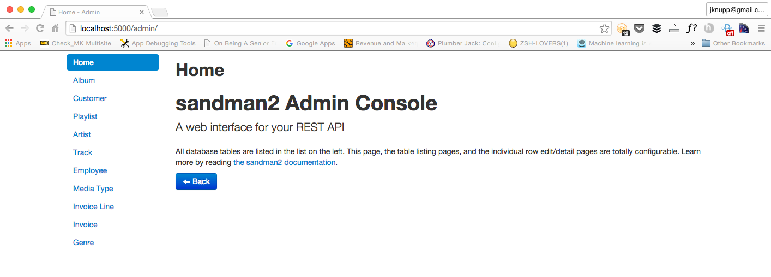
\includegraphics{images/sandman}
\caption{sandman2: Webové rozhraní \autocite{sandmanpic}\label{pic:sandman}}
\end{figure}

Sandman2 je pokračovatelem projektu sandman \autocite{sandman1}, který je momentálně opuštěný a obsahuje informaci o~tom, že by uživatelé měli používat druhou verzi \autocite{sandman1gh}. Sandman2 ale nemá tak obsáhlou dokumentaci jako sandman. Původní sandman vznikl v~roce 2013 a vyšlo celkem 45 verzí, sandman2 je zde od roku 2014, verzí vyšlo sedm, poslední v~lednu 2016. Za sandmenem stojí jednotlivec Jeff Knupp, do projektu přispělo několik jednotek dalších přispěvatelů. Na GitHubu má sandman2 pouze 128 hvězd, ale sandman jich má přes dva tisíce.

\subsection{HATEOAS}\label{hateoas}

Sandman automaticky prezentuje SQL sloupce typu cizí klíč jako odkazy \autocite{sandman1gh}. Předpokládám, že sandman2 to dělá stejně, ale tuto informaci jsem nikde nenašel potvrzenou. Dávám zde tedy dva body na základě vlastnosti z~první verze sandmanu.

\subsection{Přístupová práva}\label{pux159uxedstupovuxe1-pruxe1va}

Dokumentace k~původnímu sandmanu uvádí, že je možné použít HTTP autentizaci jménem a heslem a na základě ní zpřístupnit celé API pouze přihlášeným uživatelům \autocite{sandmanauth}. Jiné zabudované možnosti podporovány zatím nejsou. Je ale možné napsat speciální funkci, která předzpracovává všechny požadavky a v~této implementovat jiný způsob autentizace a autorizace.

Sandman2 informace o~přístupových právech v~dokumentaci neobsahuje, tato funkcionalita zde ještě není; dostává tedy nula bodů.

Sandman2 je nástroj, který mapuje REST rozhraní k~SQL databázi a dělá to dobře. Nepříjemný je přerod projektu sandman do projektu sandman2, na který doplácí hlavně dokumentace, což se doufám časem zlepší.
 \section{Tastypie}\label{tastypie}

\begin{figure}
\centering

\includegraphics{images/tastypie}
\caption{Logo Tastypie \autocite{tastypie}\label{pic:tastypie}}
\end{figure}

Tastypie je framework pro vytváření API k~webovým službám určený pro Django. Poskytuje abstrakci pro vytváření rozhraní ve stylu REST. Zjednodušuje zveřejňování modelů a umožňuje vybrat, které části budou přes API přístupné. Kromě ORM dat je možné použít i jiné zdroje. \autocite{tastypie}

Mezi hlavní funkce patří \autocite{tastypie}:

\begin{itemize}
\tightlist
\item
  podpora HTTP metod GET, POST, PUT, DELETE a PATCH,
\item
  rozumné chování ve výchozím stavu,
\item
  rozšířitelnost,
\item
  podpora různých serializačních formátů (JSON/XML/YAML/bplist),
\item
  HATEOAS,
\item
  dobré testy a dokumentace.
\end{itemize}

Projekt vznikl již v~roce 2010, od té doby vyšlo více než dvacet verzí, poslední necelý měsíc před psaním tohoto textu. Autorem projektu je jednotlivec Daniel Lindsley, který se projektu již příliš nevěnuje, v~současnosti se o~něj stará Seán Hayes, přispělo celkem více než 150 přispěvatelů. Projekt je distribuován pod permisivní BSD licencí \autocite{BSD3}.

Pokud si vystačíte s~JSON serializací, závisí Tastypie přímo na třech, nepřímo na čtyřech modulech a zabírá 41~MiB. Pro použití XML, YAML nebo bplistu je potřeba nainstalovat další moduly. Tastypie funguje na Pythonu 2 i 3 a podporuje poslední verze Djanga.

\subsection{HATEOAS}\label{hateoas}

Příklad použití můžete vidět \protect\hyperlink{code:tastypie}{v~ukázkách} \protect\hyperlink{code:tastypie2}{a}. Přímo v~tomto příkladu vznikne prolinkování mezi zdroji pomocí URL. Tastypie dostává tři body.

\begin{listing}[htbp]
\caption{{\label{code:tastypie}Příklad použití z~dokumentace Tastypie (api.py) \autocite{tastypiedoc}}}
\begin{minted}[bgcolor=codebg]{python}
from django.contrib.auth.models import User
from tastypie import fields
from tastypie.resources import ModelResource
from myapp.models import Entry


class UserResource(ModelResource):
    class Meta:
        queryset = User.objects.all()
        resource_name = 'user'


class EntryResource(ModelResource):
    user = fields.ForeignKey(UserResource, 'user')

    class Meta:
        queryset = Entry.objects.all()
        resource_name = 'entry'
\end{minted}
\end{listing}

\begin{listing}[htbp]
\caption{{\label{code:tastypie2}Příklad použití z~dokumentace Tastypie (urls.py) \autocite{tastypiedoc}}}
\begin{minted}[bgcolor=codebg]{python}
from django.conf.urls import url, include
from tastypie.api import Api
from myapp.api import EntryResource, UserResource

v1_api = Api(api_name='v1')
v1_api.register(UserResource())
v1_api.register(EntryResource())

urlpatterns = [
    # The normal jazz here...
    url(r'^blog/', include('myapp.urls')),
    url(r'^api/', include(v1_api.urls)),
]
\end{minted}
\end{listing}

\subsection{Přístupová práva}\label{pux159uxedstupovuxe1-pruxe1va}

Tastypie umožňuje autentizaci přes HTTP jméno a heslo, pomocí API klíče, session a OAuth 1; lze si také dopsat vlastní způsob \autocite{tastypieauth}. Existují moduly třetích stran přidávající podporu OAuth 2 \autocite{tastypieoath}. Na úrovni zdrojů lze pak nastavit, jaký autorizační model se použije, k~dispozici je buďto varianta povolit všechno, nebo povolit jen číst, případně lze použít propracovanější systém Djanga, který mapuje práva uživatele na konkrétní objekty; implementace vlastní logiky je také možná \autocite{tastypieauto}. I~zde tedy Tastypie získává tři body.

Tastypie se jeví jako velmi použitelný framework pro Django. Důstojně konkuruje Django REST frameworku, o~kterém jsem psal \protect\hyperlink{drf:fra}{v~části}. Případná volba mezi těmito dvěma frameworky hodně závisí na konkrétních potřebách a preferencích uživatele.


\section{Srovnání}\label{srovnuxe1nuxed}

\protect\hyperlink{tab:body}{V~tabulce} najdete udělené body za podporu HATEOASu a řízení přístupových práv.

\protect\hyperlink{tab:srovnani}{V~tabulce} najdete srovnání měřitelných kritérií. Jednotlivé sloupce mají zjednodušené názvy, ale jejich funkce odpovídá popisu \protect\hyperlink{kriteria}{v~části}. Tučně jsou označeny hodnoty, které v~daném sloupci dominují.

\protect\hyperlink{tab:informace}{V~tabulce} pak najdete informační přehled o~zkoumaných frameworcích: webový framework, URL domovské stránky a číslo zkoumané verze.

Pro implementaci si vybírám frameworky Eve a ripozo, na základě vysokého hodnocení v~oblasti HATEOAS i přístupových práv.

Vysoké hodnocení získaly i Django REST framework a Tastypie. Jelikož oba tyto frameworky rozšiřují Django, implementace v~nich by byla velmi podobná. Vybírám si proto pouze Django REST framework, který je podle indikátorů ze všech zkoumaných frameworků nejoblíbenější.

Navíc si vybírám sandman2, který nemá tak dobré hodnocení, ale slibuje automatické vytvoření API. Rád bych ze stejného důvodu zkoumal i Ramses, ale ten není možné použít s~daty v~MySQL databázi.

\begin{longtable}[]{@{}lcc@{}}

\caption{Bodové ohodnocení \label{tab:body}}\tabularnewline
\toprule
Framework & HATEOAS & Přístupová práva\tabularnewline
\midrule
\endfirsthead
\toprule
Framework & HATEOAS & Přístupová práva\tabularnewline
\midrule
\endhead
\begin{minipage}[t]{0.32\columnwidth}\raggedright\strut
Cornice\strut
\end{minipage} & \begin{minipage}[t]{0.32\columnwidth}\raggedright\strut
\strut
\end{minipage} & \begin{minipage}[t]{0.32\columnwidth}\raggedright\strut
\textbullet\strut
\end{minipage}\tabularnewline
Django REST fr. & \textbullet \textbullet \textbullet & \textbullet \textbullet \textbullet\tabularnewline
Eve & \textbullet \textbullet \textbullet & \textbullet \textbullet \textbullet\tabularnewline
\begin{minipage}[t]{0.32\columnwidth}\raggedright\strut
Falcon\strut
\end{minipage} & \begin{minipage}[t]{0.32\columnwidth}\raggedright\strut
\strut
\end{minipage} & \begin{minipage}[t]{0.32\columnwidth}\raggedright\strut
\strut
\end{minipage}\tabularnewline
\begin{minipage}[t]{0.32\columnwidth}\raggedright\strut
hug\strut
\end{minipage} & \begin{minipage}[t]{0.32\columnwidth}\raggedright\strut
\strut
\end{minipage} & \begin{minipage}[t]{0.32\columnwidth}\raggedright\strut
\textbullet \textbullet\strut
\end{minipage}\tabularnewline
\begin{minipage}[t]{0.32\columnwidth}\raggedright\strut
Flask API\strut
\end{minipage} & \begin{minipage}[t]{0.32\columnwidth}\raggedright\strut
\strut
\end{minipage} & \begin{minipage}[t]{0.32\columnwidth}\raggedright\strut
\strut
\end{minipage}\tabularnewline
\begin{minipage}[t]{0.32\columnwidth}\raggedright\strut
Flask-RESTful\strut
\end{minipage} & \begin{minipage}[t]{0.32\columnwidth}\raggedright\strut
\strut
\end{minipage} & \begin{minipage}[t]{0.32\columnwidth}\raggedright\strut
\strut
\end{minipage}\tabularnewline
Morepath & \textbullet \textbullet & \textbullet\tabularnewline
\begin{minipage}[t]{0.32\columnwidth}\raggedright\strut
Nefertari\strut
\end{minipage} & \begin{minipage}[t]{0.32\columnwidth}\raggedright\strut
\strut
\end{minipage} & \begin{minipage}[t]{0.32\columnwidth}\raggedright\strut
\textbullet\strut
\end{minipage}\tabularnewline
\begin{minipage}[t]{0.32\columnwidth}\raggedright\strut
Ramses\strut
\end{minipage} & \begin{minipage}[t]{0.32\columnwidth}\raggedright\strut
\strut
\end{minipage} & \begin{minipage}[t]{0.32\columnwidth}\raggedright\strut
\textbullet\strut
\end{minipage}\tabularnewline
\begin{minipage}[t]{0.32\columnwidth}\raggedright\strut
Piston\strut
\end{minipage} & \begin{minipage}[t]{0.32\columnwidth}\raggedright\strut
\strut
\end{minipage} & \begin{minipage}[t]{0.32\columnwidth}\raggedright\strut
\textbullet \textbullet \textbullet\strut
\end{minipage}\tabularnewline
\begin{minipage}[t]{0.32\columnwidth}\raggedright\strut
Pycnic\strut
\end{minipage} & \begin{minipage}[t]{0.32\columnwidth}\raggedright\strut
\strut
\end{minipage} & \begin{minipage}[t]{0.32\columnwidth}\raggedright\strut
\strut
\end{minipage}\tabularnewline
Python REST API fr. & \textbullet & \textbullet \textbullet\tabularnewline
RESTArt & \textbullet & \textbullet\tabularnewline
\begin{minipage}[t]{0.32\columnwidth}\raggedright\strut
restless\strut
\end{minipage} & \begin{minipage}[t]{0.32\columnwidth}\raggedright\strut
\strut
\end{minipage} & \begin{minipage}[t]{0.32\columnwidth}\raggedright\strut
\strut
\end{minipage}\tabularnewline
ripozo & \textbullet \textbullet \textbullet & \textbullet \textbullet\tabularnewline
\begin{minipage}[t]{0.32\columnwidth}\raggedright\strut
sandman2\strut
\end{minipage} & \begin{minipage}[t]{0.32\columnwidth}\raggedright\strut
\textbullet \textbullet\strut
\end{minipage} & \begin{minipage}[t]{0.32\columnwidth}\raggedright\strut
\strut
\end{minipage}\tabularnewline
Tastypie & \textbullet \textbullet \textbullet & \textbullet \textbullet \textbullet\tabularnewline
\bottomrule
\end{longtable}

\begin{landscape}
\begin{longtable}[]{@{}lllrrrrrrr@{}}

\caption{Srovnání měřitelných kritérií \label{tab:srovnani}}\tabularnewline
\toprule
Framework & Druh licence & Webový fr. & MiB & Řádky & Ř. včetně & Závisl. & Py & GitHub & PyPI\tabularnewline
\midrule
\endfirsthead
\toprule
Framework & Druh licence & Webový fr. & MiB & Řádky & Ř. včetně & Závisl. & Py & GitHub & PyPI\tabularnewline
\midrule
\endhead
Cornice & LGPL & lightweight & 12 & 1 198 & 24 625 & 2/9 & \textbf{3+2} & 270 & 10 903\tabularnewline
Django REST fr. & \textbf{permisivní} & MVC & 43 & 7 057 & 79 854 & 1/1 & \textbf{3+2} & \textbf{5 606} & \textbf{316 772}\tabularnewline
Eve & \textbf{permisivní} & lightweight & 10 & 3 440 & 35 009 & 10/10 & \textbf{3+2} & 3 121 & 7 480\tabularnewline
Falcon & \textbf{permisivní} & \textbf{standalone} & 0,9 & 2 352 & 3 034 & 2/2 & \textbf{3+2} & 2 756 & 51 071\tabularnewline
hug & \textbf{permisivní} & lightweight & 4 & 2 367 & 16 545 & 2/4 & 3 & 3 020 & 7 674\tabularnewline
Flask API & \textbf{permisivní} & lightweight & 6 & 620 & 20 938 & 1/5 & \textbf{3+2} & 688 & 7 594\tabularnewline
Flask-RESTful & \textbf{permisivní} & lightweight & 9 & 967 & 27 718 & 4/9 & \textbf{3+2} & 1 920 & 172 775\tabularnewline
Morepath & \textbf{permisivní} & \textbf{standalone} & 4 & 1 940 & 9 156 & 4/5 & \textbf{3+2} & 226 & 1 594\tabularnewline
Nefertari & \textbf{permisivní} & lightweight & 16 & 2 905 & 54 339 & 9/18 & \textbf{3+2} & 37 & 812\tabularnewline
Ramses & \textbf{permisivní} & lightweight & 19 & 1 067 & 68 594 & 7/29 & \textbf{3+2} & 216 & 661\tabularnewline
Piston & \textbf{permisivní} & MVC & 49 & 1 935 & 75 311 & 1/1 & 2 & -- & 2 419\tabularnewline
Pycnic & \textbf{permisivní} & \textbf{standalone} & \textbf{0,08} & \textbf{226} & \textbf{226} & \textbf{0/0} & \textbf{3+2} & 33 & 304\tabularnewline
Python REST API fr. & \textbf{permisivní} & lightweight & 3 & 954 & 15 988 & 2/3 & 2 & 4 & 248\tabularnewline
RESTArt & \textbf{permisivní} & lightweight & 3 & 798 & 20 105 & 4/5 & \textbf{3+2} & 10 & 829\tabularnewline
restless & \textbf{permisivní} & lightw./MVC & \(\geq\) 0,25 & 528 & \(\geq\) 1 140 & \(\geq\) 1/1 & \textbf{3+2} & 520 & 7 909\tabularnewline
ripozo & copyleft & lightw./MVC & \(\geq\) 0,5 & 1 518 & \(\geq\) 2 130 & \(\geq\) 1/1 & \textbf{3+2} & 151 & 2 411\tabularnewline
sandman2 & \textbf{permisivní} & lightweight & 23 & 446 & 82 207 & 4/12 & \textbf{3+2} & 128 & 625\tabularnewline
Tastypie & \textbf{permisivní} & MVC & 41 & 3 292 & 80 139 & 3/4 & \textbf{3+2} & 2 940 & 28 966\tabularnewline
\bottomrule
\end{longtable}
\end{landscape}

\begin{landscape}
\begin{longtable}[]{@{}lllr@{}}

\caption{Informace o~frameworcích \label{tab:informace}}\tabularnewline
\toprule
Framework & Webový fr. & Webová stránka & Zk. verze\tabularnewline
\midrule
\endfirsthead
\toprule
Framework & Webový fr. & Webová stránka & Zk. verze\tabularnewline
\midrule
\endhead
Cornice & Pyramid & \url{https://cornice.readthedocs.org/} & 1.2.1\tabularnewline
Django REST fr. & Django & \url{http://www.django-rest-framework.org/} & 3.3.3\tabularnewline
Eve & Flask & \url{http://python-eve.org/} & 0.6.3\tabularnewline
Falcon & -- & \url{http://falconframework.org/} & 0.3.0\tabularnewline
hug & Falcon & \url{http://www.hug.rest/} & 2.0.6\tabularnewline
Flask API & Flask & \url{http://www.flaskapi.org/} & 0.6.5\tabularnewline
Flask-RESTful & Flask & \url{https://flask-restful.readthedocs.org/} & 0.3.5\tabularnewline
Morepath & -- & \url{https://morepath.readthedocs.org/} & 0.13\tabularnewline
Nefertari & Pyramid & \url{https://nefertari.readthedocs.org/} & 0.6.1\tabularnewline
Ramses & Pyramid & \url{http://ramses.tech/} & 0.5.1\tabularnewline
Piston & Django & \url{https://bitbucket.org/jespern/django-piston/} & 0.2.3\tabularnewline
Pycnic & -- & \url{http://pycnic.nullism.com/} & 0.0.5\tabularnewline
Python REST API fr. & Werkzeug & \url{https://python-rest-framework.readthedocs.org/} & 1.3\tabularnewline
RESTArt & Werkzeug & \url{https://restart.readthedocs.org/} & 0.1.3\tabularnewline
restless & \emph{volitelný} & \url{https://restless.readthedocs.org/} & 2.0.1\tabularnewline
ripozo & \emph{volitelný} & \url{https://ripozo.readthedocs.org/} & 1.3.0\tabularnewline
sandman2 & Flask & \url{http://pythonhosted.org/sandman2/} & 0.0.7\tabularnewline
Tastypie & Django & \url{http://tastypieapi.org/} & 0.13.3\tabularnewline
\bottomrule
\end{longtable}
\end{landscape}
